\documentclass[twoside]{book}

% Packages required by doxygen
\usepackage{calc}
\usepackage{doxygen}
\usepackage{graphicx}
\usepackage[utf8]{inputenc}
\usepackage{makeidx}
\usepackage{multicol}
\usepackage{multirow}
\usepackage{textcomp}
\usepackage[table]{xcolor}

% NLS support packages
\usepackage[ngerman]{babel}

% Font selection
\usepackage[T1]{fontenc}
\usepackage{mathptmx}
\usepackage[scaled=.90]{helvet}
\usepackage{courier}
\usepackage{amssymb}
\usepackage{sectsty}
\renewcommand{\familydefault}{\sfdefault}
\allsectionsfont{%
  \fontseries{bc}\selectfont%
  \color{darkgray}%
}
\renewcommand{\DoxyLabelFont}{%
  \fontseries{bc}\selectfont%
  \color{darkgray}%
}

% Page & text layout
\usepackage{geometry}
\geometry{%
  a4paper,%
  top=2.5cm,%
  bottom=2.5cm,%
  left=2.5cm,%
  right=2.5cm%
}
\tolerance=750
\hfuzz=15pt
\hbadness=750
\setlength{\emergencystretch}{15pt}
\setlength{\parindent}{0cm}
\setlength{\parskip}{0.2cm}
\makeatletter
\renewcommand{\paragraph}{%
  \@startsection{paragraph}{4}{0ex}{-1.0ex}{1.0ex}{%
    \normalfont\normalsize\bfseries\SS@parafont%
  }%
}
\renewcommand{\subparagraph}{%
  \@startsection{subparagraph}{5}{0ex}{-1.0ex}{1.0ex}{%
    \normalfont\normalsize\bfseries\SS@subparafont%
  }%
}
\makeatother

% Headers & footers
\usepackage{fancyhdr}
\pagestyle{fancyplain}
\fancyhead[LE]{\fancyplain{}{\bfseries\thepage}}
\fancyhead[CE]{\fancyplain{}{}}
\fancyhead[RE]{\fancyplain{}{\bfseries\leftmark}}
\fancyhead[LO]{\fancyplain{}{\bfseries\rightmark}}
\fancyhead[CO]{\fancyplain{}{}}
\fancyhead[RO]{\fancyplain{}{\bfseries\thepage}}
\fancyfoot[LE]{\fancyplain{}{}}
\fancyfoot[CE]{\fancyplain{}{}}
\fancyfoot[RE]{\fancyplain{}{\bfseries\scriptsize Erzeugt am Don Aug 29 2013 08\-:47\-:03 für D\-B\-A02 von Doxygen }}
\fancyfoot[LO]{\fancyplain{}{\bfseries\scriptsize Erzeugt am Don Aug 29 2013 08\-:47\-:03 für D\-B\-A02 von Doxygen }}
\fancyfoot[CO]{\fancyplain{}{}}
\fancyfoot[RO]{\fancyplain{}{}}
\renewcommand{\footrulewidth}{0.4pt}
\renewcommand{\chaptermark}[1]{%
  \markboth{#1}{}%
}
\renewcommand{\sectionmark}[1]{%
  \markright{\thesection\ #1}%
}

% Indices & bibliography
\usepackage{natbib}
\usepackage[titles]{tocloft}
\setcounter{tocdepth}{3}
\setcounter{secnumdepth}{5}
\makeindex

% Hyperlinks (required, but should be loaded last)
\usepackage{ifpdf}
\ifpdf
  \usepackage[pdftex,pagebackref=true]{hyperref}
\else
  \usepackage[ps2pdf,pagebackref=true]{hyperref}
\fi
\hypersetup{%
  colorlinks=true,%
  linkcolor=blue,%
  citecolor=blue,%
  unicode%
}

% Custom commands
\newcommand{\clearemptydoublepage}{%
  \newpage{\pagestyle{empty}\cleardoublepage}%
}


%===== C O N T E N T S =====

\begin{document}

% Titlepage & ToC
\hypersetup{pageanchor=false}
\pagenumbering{roman}
\begin{titlepage}
\vspace*{7cm}
\begin{center}%
{\Large D\-B\-A02 }\\
\vspace*{1cm}
{\large Erzeugt von Doxygen 1.8.5}\\
\vspace*{0.5cm}
{\small Don Aug 29 2013 08:47:03}\\
\end{center}
\end{titlepage}
\clearemptydoublepage
\tableofcontents
\clearemptydoublepage
\pagenumbering{arabic}
\hypersetup{pageanchor=true}

%--- Begin generated contents ---
\chapter{Hierarchie-\/\-Verzeichnis}
\section{Klassenhierarchie}
Die Liste der Ableitungen ist -\/mit Einschränkungen-\/ alphabetisch sortiert\-:\begin{DoxyCompactList}
\item \contentsline{section}{Controller\textbackslash{}Admin\textbackslash{}Base}{\pageref{class_controller_1_1_admin_1_1_base}}{}
\begin{DoxyCompactList}
\item \contentsline{section}{Controller\textbackslash{}Admin\textbackslash{}Stats}{\pageref{class_controller_1_1_admin_1_1_stats}}{}
\item \contentsline{section}{Controller\textbackslash{}Admin\textbackslash{}Survey}{\pageref{class_controller_1_1_admin_1_1_survey}}{}
\item \contentsline{section}{Controller\textbackslash{}Admin\textbackslash{}User}{\pageref{class_controller_1_1_admin_1_1_user}}{}
\end{DoxyCompactList}
\item \contentsline{section}{Model\textbackslash{}Base}{\pageref{class_model_1_1_base}}{}
\begin{DoxyCompactList}
\item \contentsline{section}{Model\textbackslash{}Survey}{\pageref{class_model_1_1_survey}}{}
\item \contentsline{section}{Model\textbackslash{}User}{\pageref{class_model_1_1_user}}{}
\end{DoxyCompactList}
\item \contentsline{section}{Config}{\pageref{class_config}}{}
\item \contentsline{section}{Controller\textbackslash{}Database}{\pageref{class_controller_1_1_database}}{}
\item Exception\begin{DoxyCompactList}
\item \contentsline{section}{Custom\-Exception\textbackslash{}Invalid\-User\-Pass\-Exception}{\pageref{class_custom_exception_1_1_invalid_user_pass_exception}}{}
\item \contentsline{section}{Custom\-Exception\textbackslash{}User\-Not\-Authed\-Exception}{\pageref{class_custom_exception_1_1_user_not_authed_exception}}{}
\end{DoxyCompactList}
\item \contentsline{section}{Front\-Controller}{\pageref{class_front_controller}}{}
\item \contentsline{section}{Controller\textbackslash{}Index}{\pageref{class_controller_1_1_index}}{}
\item P\-D\-O\begin{DoxyCompactList}
\item \contentsline{section}{Database}{\pageref{class_database}}{}
\end{DoxyCompactList}
\item \contentsline{section}{Redirect}{\pageref{class_redirect}}{}
\item \contentsline{section}{Session}{\pageref{class_session}}{}
\item \contentsline{section}{Controller\textbackslash{}Survey}{\pageref{class_controller_1_1_survey}}{}
\item \contentsline{section}{Controller\textbackslash{}User\-Session}{\pageref{class_controller_1_1_user_session}}{}
\item \contentsline{section}{View}{\pageref{class_view}}{}
\end{DoxyCompactList}

\chapter{Klassen-\/\-Verzeichnis}
\section{Auflistung der Klassen}
Hier folgt die Aufzählung aller Klassen, Strukturen, Varianten und Schnittstellen mit einer Kurzbeschreibung\-:\begin{DoxyCompactList}
\item\contentsline{section}{\hyperlink{class_controller_1_1_admin_1_1_base}{Controller\textbackslash{}\-Admin\textbackslash{}\-Base} }{\pageref{class_controller_1_1_admin_1_1_base}}{}
\item\contentsline{section}{\hyperlink{class_model_1_1_base}{Model\textbackslash{}\-Base} }{\pageref{class_model_1_1_base}}{}
\item\contentsline{section}{\hyperlink{class_config}{Config} }{\pageref{class_config}}{}
\item\contentsline{section}{\hyperlink{class_database}{Database} }{\pageref{class_database}}{}
\item\contentsline{section}{\hyperlink{class_controller_1_1_database}{Controller\textbackslash{}\-Database} }{\pageref{class_controller_1_1_database}}{}
\item\contentsline{section}{\hyperlink{class_front_controller}{Front\-Controller} }{\pageref{class_front_controller}}{}
\item\contentsline{section}{\hyperlink{class_controller_1_1_index}{Controller\textbackslash{}\-Index} }{\pageref{class_controller_1_1_index}}{}
\item\contentsline{section}{\hyperlink{class_custom_exception_1_1_invalid_user_pass_exception}{Custom\-Exception\textbackslash{}\-Invalid\-User\-Pass\-Exception} }{\pageref{class_custom_exception_1_1_invalid_user_pass_exception}}{}
\item\contentsline{section}{\hyperlink{class_redirect}{Redirect} }{\pageref{class_redirect}}{}
\item\contentsline{section}{\hyperlink{class_session}{Session} }{\pageref{class_session}}{}
\item\contentsline{section}{\hyperlink{class_controller_1_1_admin_1_1_stats}{Controller\textbackslash{}\-Admin\textbackslash{}\-Stats} }{\pageref{class_controller_1_1_admin_1_1_stats}}{}
\item\contentsline{section}{\hyperlink{class_controller_1_1_admin_1_1_survey}{Controller\textbackslash{}\-Admin\textbackslash{}\-Survey} }{\pageref{class_controller_1_1_admin_1_1_survey}}{}
\item\contentsline{section}{\hyperlink{class_controller_1_1_survey}{Controller\textbackslash{}\-Survey} }{\pageref{class_controller_1_1_survey}}{}
\item\contentsline{section}{\hyperlink{class_model_1_1_survey}{Model\textbackslash{}\-Survey} }{\pageref{class_model_1_1_survey}}{}
\item\contentsline{section}{\hyperlink{class_model_1_1_user}{Model\textbackslash{}\-User} }{\pageref{class_model_1_1_user}}{}
\item\contentsline{section}{\hyperlink{class_controller_1_1_admin_1_1_user}{Controller\textbackslash{}\-Admin\textbackslash{}\-User} }{\pageref{class_controller_1_1_admin_1_1_user}}{}
\item\contentsline{section}{\hyperlink{class_custom_exception_1_1_user_not_authed_exception}{Custom\-Exception\textbackslash{}\-User\-Not\-Authed\-Exception} }{\pageref{class_custom_exception_1_1_user_not_authed_exception}}{}
\item\contentsline{section}{\hyperlink{class_controller_1_1_user_session}{Controller\textbackslash{}\-User\-Session} }{\pageref{class_controller_1_1_user_session}}{}
\item\contentsline{section}{\hyperlink{class_view}{View} }{\pageref{class_view}}{}
\end{DoxyCompactList}

\chapter{Klassen-\/\-Dokumentation}
\hypertarget{class_controller_1_1_admin_1_1_base}{\section{Controller\textbackslash{}Admin\textbackslash{}Base Klassenreferenz}
\label{class_controller_1_1_admin_1_1_base}\index{Controller\textbackslash{}\-Admin\textbackslash{}\-Base@{Controller\textbackslash{}\-Admin\textbackslash{}\-Base}}
}
Klassendiagramm für Controller\textbackslash{}Admin\textbackslash{}Base\-:\begin{figure}[H]
\begin{center}
\leavevmode
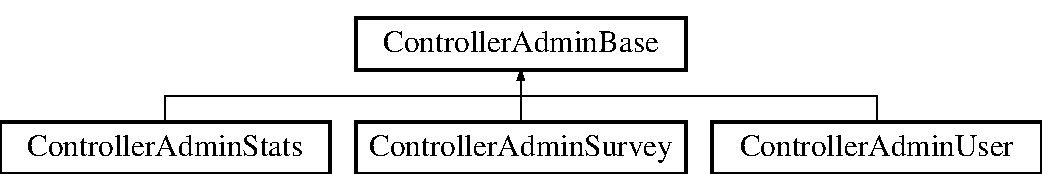
\includegraphics[height=2.000000cm]{class_controller_1_1_admin_1_1_base}
\end{center}
\end{figure}
\subsection*{Öffentliche Methoden}
\begin{DoxyCompactItemize}
\item 
\hyperlink{class_controller_1_1_admin_1_1_base_a7e433734833c21c222186860f4cd8ce5}{\-\_\-\-\_\-construct} ()
\end{DoxyCompactItemize}


\subsection{Ausführliche Beschreibung}
Admin \hyperlink{class_controller_1_1_admin_1_1_base}{Base} Controller 

Definiert in Zeile \hyperlink{_controller_2_admin_2_base_8php_source_l00010}{10} der Datei \hyperlink{_controller_2_admin_2_base_8php_source}{Controller/\-Admin/\-Base.\-php}.



\subsection{Beschreibung der Konstruktoren und Destruktoren}
\hypertarget{class_controller_1_1_admin_1_1_base_a7e433734833c21c222186860f4cd8ce5}{\index{Controller\-::\-Admin\-::\-Base@{Controller\-::\-Admin\-::\-Base}!\-\_\-\-\_\-construct@{\-\_\-\-\_\-construct}}
\index{\-\_\-\-\_\-construct@{\-\_\-\-\_\-construct}!Controller::Admin::Base@{Controller\-::\-Admin\-::\-Base}}
\subsubsection[{\-\_\-\-\_\-construct}]{\setlength{\rightskip}{0pt plus 5cm}Controller\textbackslash{}\-Admin\textbackslash{}\-Base\-::\-\_\-\-\_\-construct (
\begin{DoxyParamCaption}
{}
\end{DoxyParamCaption}
)}}\label{class_controller_1_1_admin_1_1_base_a7e433734833c21c222186860f4cd8ce5}
Im Konstruktur generell ueberpruefen ob sich der \hyperlink{class_controller_1_1_admin_1_1_user}{User} eingeloggt hat. 

Definiert in Zeile \hyperlink{_controller_2_admin_2_base_8php_source_l00018}{18} der Datei \hyperlink{_controller_2_admin_2_base_8php_source}{Controller/\-Admin/\-Base.\-php}.


\begin{DoxyCode}
00018                                       \{
00019                 
00020                 \hyperlink{class_session_a49f0fb7185ab07bdbf6bdff477b43ff8}{\(\backslash\)Session::isUserAuthedCheck}();
00021                 
00022         \}
\end{DoxyCode}


Die Dokumentation für diese Klasse wurde erzeugt aufgrund der Datei\-:\begin{DoxyCompactItemize}
\item 
Controller/\-Admin/\-Base.\-php\end{DoxyCompactItemize}

\hypertarget{class_model_1_1_base}{\section{Model\textbackslash{}Base Klassenreferenz}
\label{class_model_1_1_base}\index{Model\textbackslash{}\-Base@{Model\textbackslash{}\-Base}}
}
Klassendiagramm für Model\textbackslash{}Base\-:\begin{figure}[H]
\begin{center}
\leavevmode
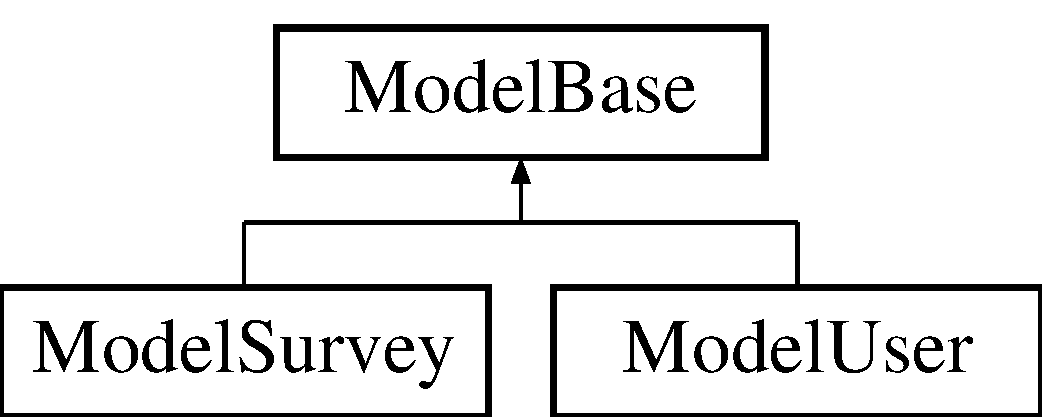
\includegraphics[height=2.000000cm]{class_model_1_1_base}
\end{center}
\end{figure}
\subsection*{Öffentliche Methoden}
\begin{DoxyCompactItemize}
\item 
\hyperlink{class_model_1_1_base_a72e3b51dec693b4a3f33f445e837d7e8}{\-\_\-\-\_\-construct} ()
\end{DoxyCompactItemize}
\subsection*{Geschützte Attribute}
\begin{DoxyCompactItemize}
\item 
\hypertarget{class_model_1_1_base_a10c7d143c93e0976d53f9e5ab126b1c4}{{\bfseries \$dbh}}\label{class_model_1_1_base_a10c7d143c93e0976d53f9e5ab126b1c4}

\end{DoxyCompactItemize}


\subsection{Ausführliche Beschreibung}
Basis Datenmodell 

Definiert in Zeile \hyperlink{_model_2_base_8php_source_l00009}{9} der Datei \hyperlink{_model_2_base_8php_source}{Model/\-Base.\-php}.



\subsection{Beschreibung der Konstruktoren und Destruktoren}
\hypertarget{class_model_1_1_base_a72e3b51dec693b4a3f33f445e837d7e8}{\index{Model\-::\-Base@{Model\-::\-Base}!\-\_\-\-\_\-construct@{\-\_\-\-\_\-construct}}
\index{\-\_\-\-\_\-construct@{\-\_\-\-\_\-construct}!Model::Base@{Model\-::\-Base}}
\subsubsection[{\-\_\-\-\_\-construct}]{\setlength{\rightskip}{0pt plus 5cm}Model\textbackslash{}\-Base\-::\-\_\-\-\_\-construct (
\begin{DoxyParamCaption}
{}
\end{DoxyParamCaption}
)}}\label{class_model_1_1_base_a72e3b51dec693b4a3f33f445e837d7e8}
Konstruktor

Datenbank Verbindung herstellen. 

Definiert in Zeile \hyperlink{_model_2_base_8php_source_l00021}{21} der Datei \hyperlink{_model_2_base_8php_source}{Model/\-Base.\-php}.


\begin{DoxyCode}
00021                                       \{
00022                 
00023                 $this->dbh = new \(\backslash\)Database();
00024                 
00025         \}
\end{DoxyCode}


Die Dokumentation für diese Klasse wurde erzeugt aufgrund der Datei\-:\begin{DoxyCompactItemize}
\item 
Model/\-Base.\-php\end{DoxyCompactItemize}

\hypertarget{class_config}{\section{Config Klassenreferenz}
\label{class_config}\index{Config@{Config}}
}
\subsection*{Öffentliche Methoden}
\begin{DoxyCompactItemize}
\item 
\hyperlink{class_config_aeb4233e287af07c75fff2d77e28a1eba}{\-\_\-\-\_\-get} (\$key)
\end{DoxyCompactItemize}
\subsection*{Öffentliche, statische Methoden}
\begin{DoxyCompactItemize}
\item 
\hypertarget{class_config_aef7aac9c02b60638561fe777a87a5673}{static {\bfseries get\-Instance} ()}\label{class_config_aef7aac9c02b60638561fe777a87a5673}

\end{DoxyCompactItemize}
\subsection*{Private Methoden}
\begin{DoxyCompactItemize}
\item 
\hyperlink{class_config_ac1c75b1b53a17a028629ba8127e06f82}{\-\_\-\-\_\-construct} ()
\item 
\hypertarget{class_config_aa84beb1afac47a0723dbfa5be7e6be72}{{\bfseries \-\_\-\-\_\-clone} ()}\label{class_config_aa84beb1afac47a0723dbfa5be7e6be72}

\end{DoxyCompactItemize}
\subsection*{Private Attribute}
\begin{DoxyCompactItemize}
\item 
\hypertarget{class_config_abdb13aa29fd63a731b31ba0e709c7faa}{{\bfseries \$config} = array()}\label{class_config_abdb13aa29fd63a731b31ba0e709c7faa}

\end{DoxyCompactItemize}
\subsection*{Statische, private Attribute}
\begin{DoxyCompactItemize}
\item 
\hypertarget{class_config_ac75489237154302980c51f1d1464d0af}{static {\bfseries \$instance} = null}\label{class_config_ac75489237154302980c51f1d1464d0af}

\end{DoxyCompactItemize}


\subsection{Ausführliche Beschreibung}
\hyperlink{class_config}{Config} Klasse als Singleton Pattern

\$conf = \-::get\-Instance(); \$value = \$conf-\/$>$key;

Die Werte stehen in der Ini Datei und koennen direkt abgerufen werden. 

Definiert in Zeile \hyperlink{_config_8php_source_l00013}{13} der Datei \hyperlink{_config_8php_source}{Config.\-php}.



\subsection{Beschreibung der Konstruktoren und Destruktoren}
\hypertarget{class_config_ac1c75b1b53a17a028629ba8127e06f82}{\index{Config@{Config}!\-\_\-\-\_\-construct@{\-\_\-\-\_\-construct}}
\index{\-\_\-\-\_\-construct@{\-\_\-\-\_\-construct}!Config@{Config}}
\subsubsection[{\-\_\-\-\_\-construct}]{\setlength{\rightskip}{0pt plus 5cm}Config\-::\-\_\-\-\_\-construct (
\begin{DoxyParamCaption}
{}
\end{DoxyParamCaption}
)\hspace{0.3cm}{\ttfamily [private]}}}\label{class_config_ac1c75b1b53a17a028629ba8127e06f82}
Konstruktor

Wird nur einmal aufgerufen wegen Singleton Pattern

Konfigurationsdatei einlesen 

Definiert in Zeile \hyperlink{_config_8php_source_l00036}{36} der Datei \hyperlink{_config_8php_source}{Config.\-php}.


\begin{DoxyCode}
00036                                        \{
00037                 $this->config = parse\_ini\_file(CONFIGFILE);
00038         \}
\end{DoxyCode}


\subsection{Dokumentation der Elementfunktionen}
\hypertarget{class_config_aeb4233e287af07c75fff2d77e28a1eba}{\index{Config@{Config}!\-\_\-\-\_\-get@{\-\_\-\-\_\-get}}
\index{\-\_\-\-\_\-get@{\-\_\-\-\_\-get}!Config@{Config}}
\subsubsection[{\-\_\-\-\_\-get}]{\setlength{\rightskip}{0pt plus 5cm}Config\-::\-\_\-\-\_\-get (
\begin{DoxyParamCaption}
\item[{}]{\$key}
\end{DoxyParamCaption}
)}}\label{class_config_aeb4233e287af07c75fff2d77e28a1eba}
Getter Methode


\begin{DoxyParams}[1]{Parameter}
String & {\em \$key} & Schlüssel\\
\hline
\end{DoxyParams}
\begin{DoxyReturn}{Rückgabe}
String Wert 
\end{DoxyReturn}


Definiert in Zeile \hyperlink{_config_8php_source_l00051}{51} der Datei \hyperlink{_config_8php_source}{Config.\-php}.


\begin{DoxyCode}
00051                                     \{
00052                                 
00053                 \textcolor{keywordflow}{if} (array\_key\_exists($key, $this->config)) \{
00054                         \textcolor{keywordflow}{return} $this->config[$key];
00055                 \} \textcolor{keywordflow}{else} \{
00056                         \textcolor{keywordflow}{throw} \textcolor{keyword}{new} Exception(\textcolor{stringliteral}{"Config Schluessel '$key' nicht verfuegbar"});
00057                 \}
00058                 
00059         \}
\end{DoxyCode}


Die Dokumentation für diese Klasse wurde erzeugt aufgrund der Datei\-:\begin{DoxyCompactItemize}
\item 
Config.\-php\end{DoxyCompactItemize}

\hypertarget{class_database}{\section{Database Klassenreferenz}
\label{class_database}\index{Database@{Database}}
}
Klassendiagramm für Database\-:\begin{figure}[H]
\begin{center}
\leavevmode
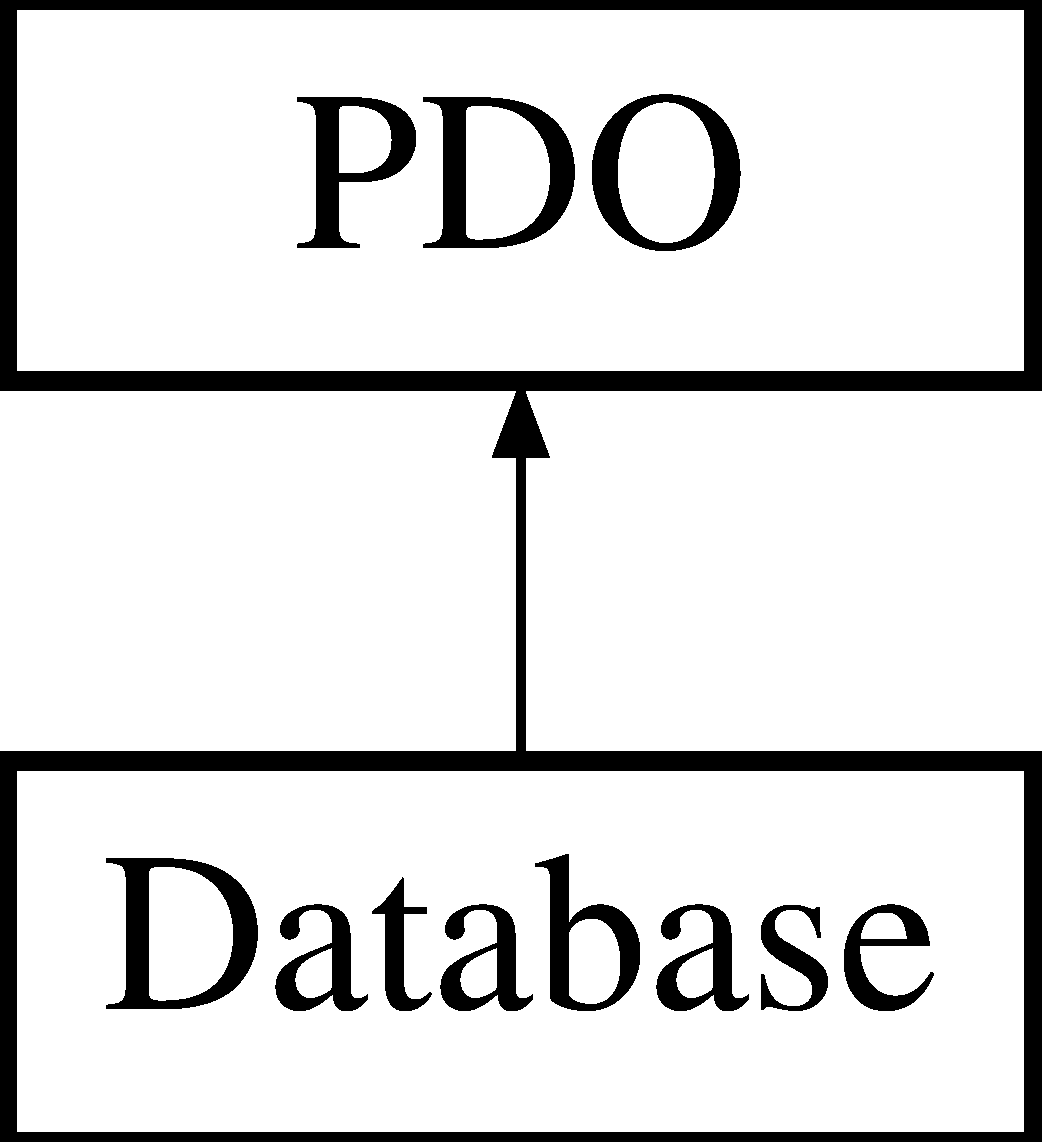
\includegraphics[height=2.000000cm]{class_database}
\end{center}
\end{figure}
\subsection*{Öffentliche Methoden}
\begin{DoxyCompactItemize}
\item 
\hyperlink{class_database_a2852f635197e76a838486e64e00aac9f}{\-\_\-\-\_\-construct} ()
\end{DoxyCompactItemize}
\subsection*{Private Methoden}
\begin{DoxyCompactItemize}
\item 
\hypertarget{class_database_a669fc0eb6ea0dc6bb76411e0338886c7}{{\bfseries be\-More\-Verbose} ()}\label{class_database_a669fc0eb6ea0dc6bb76411e0338886c7}

\end{DoxyCompactItemize}
\subsection*{Private Attribute}
\begin{DoxyCompactItemize}
\item 
\hypertarget{class_database_acf4bc044b7d1c3e54536ea4f2b0da56a}{{\bfseries \$dsn}}\label{class_database_acf4bc044b7d1c3e54536ea4f2b0da56a}

\item 
\hypertarget{class_database_ae9e43fb2a274428ec75ae70be7ab045f}{{\bfseries \$user}}\label{class_database_ae9e43fb2a274428ec75ae70be7ab045f}

\item 
\hypertarget{class_database_a8783a2890064e9d86b48a55fa09432f5}{{\bfseries \$pass}}\label{class_database_a8783a2890064e9d86b48a55fa09432f5}

\end{DoxyCompactItemize}


\subsection{Ausführliche Beschreibung}
\hyperlink{class_database}{Database} Klasse erweitert P\-H\-P P\-D\-O

\$db = new \hyperlink{class_database}{Database()}; 

Definiert in Zeile \hyperlink{_database_8php_source_l00009}{9} der Datei \hyperlink{_database_8php_source}{Database.\-php}.



\subsection{Beschreibung der Konstruktoren und Destruktoren}
\hypertarget{class_database_a2852f635197e76a838486e64e00aac9f}{\index{Database@{Database}!\-\_\-\-\_\-construct@{\-\_\-\-\_\-construct}}
\index{\-\_\-\-\_\-construct@{\-\_\-\-\_\-construct}!Database@{Database}}
\subsubsection[{\-\_\-\-\_\-construct}]{\setlength{\rightskip}{0pt plus 5cm}Database\-::\-\_\-\-\_\-construct (
\begin{DoxyParamCaption}
{}
\end{DoxyParamCaption}
)}}\label{class_database_a2852f635197e76a838486e64e00aac9f}
Konstruktor.

Konfiguration laden und der Elternklasse uebergeben. 

Definiert in Zeile \hyperlink{_database_8php_source_l00022}{22} der Datei \hyperlink{_database_8php_source}{Database.\-php}.


\begin{DoxyCode}
00022                                       \{
00023                 
00024                 $conf = \(\backslash\)Config::getInstance();
00025 
00026                 $this->dsn = $conf->database\_type . \textcolor{stringliteral}{":host="} . $conf->database\_host . \textcolor{stringliteral}{";port="} . $conf->
      database\_port . \textcolor{stringliteral}{";dbname="} . $conf->database\_name; 
00027                 
00028                 $this->user = $conf->database\_user;
00029                 $this->pass = $conf->database\_pass;
00030 
00031                 parent::\_\_construct($this->dsn, $this->user, $this->pass);
00032 
00033         
00034         \textcolor{keywordflow}{if} ($conf->database\_verbose == 1) $this->beMoreVerbose(); 
00035         
00036                 
00037         \}
\end{DoxyCode}


Die Dokumentation für diese Klasse wurde erzeugt aufgrund der Datei\-:\begin{DoxyCompactItemize}
\item 
Database.\-php\end{DoxyCompactItemize}

\hypertarget{class_front_controller}{\section{Front\-Controller Klassenreferenz}
\label{class_front_controller}\index{Front\-Controller@{Front\-Controller}}
}
\subsection*{Öffentliche Methoden}
\begin{DoxyCompactItemize}
\item 
\hyperlink{class_front_controller_ad0793ef177eb6e77a45a476567b531b2}{\-\_\-\-\_\-construct} ()
\item 
\hyperlink{class_front_controller_aee82b9818875d037d6312b856f76403c}{run} ()
\end{DoxyCompactItemize}
\subsection*{Private Attribute}
\begin{DoxyCompactItemize}
\item 
\hypertarget{class_front_controller_ac37e637f55efd166dfcce76240310cd3}{{\bfseries \$controller}}\label{class_front_controller_ac37e637f55efd166dfcce76240310cd3}

\item 
\hypertarget{class_front_controller_a281612757251bf7b0398826d6d9e1450}{{\bfseries \$action}}\label{class_front_controller_a281612757251bf7b0398826d6d9e1450}

\end{DoxyCompactItemize}


\subsection{Ausführliche Beschreibung}
\hyperlink{class_front_controller}{Front\-Controller} Klasse

Get Request\-: ?controller=test\&action=machwas

Ergebsniss\-: Automatisches Einbinden der Controllerklasse \char`\"{}test\char`\"{} und Aufruf der Methode machwas\-\_\-\-Action()

Beim gleichen Request als Post wird die Methode machwas\-\_\-\-Action\-\_\-\-P\-O\-S\-T() aufgerufen 

Definiert in Zeile \hyperlink{_front_controller_8php_source_l00018}{18} der Datei \hyperlink{_front_controller_8php_source}{Front\-Controller.\-php}.



\subsection{Beschreibung der Konstruktoren und Destruktoren}
\hypertarget{class_front_controller_ad0793ef177eb6e77a45a476567b531b2}{\index{Front\-Controller@{Front\-Controller}!\-\_\-\-\_\-construct@{\-\_\-\-\_\-construct}}
\index{\-\_\-\-\_\-construct@{\-\_\-\-\_\-construct}!FrontController@{Front\-Controller}}
\subsubsection[{\-\_\-\-\_\-construct}]{\setlength{\rightskip}{0pt plus 5cm}Front\-Controller\-::\-\_\-\-\_\-construct (
\begin{DoxyParamCaption}
{}
\end{DoxyParamCaption}
)}}\label{class_front_controller_ad0793ef177eb6e77a45a476567b531b2}
Konstruktor

\$c = new Front\-Crontroller() \$c-\/$>$\hyperlink{class_front_controller_aee82b9818875d037d6312b856f76403c}{run()}; 

Definiert in Zeile \hyperlink{_front_controller_8php_source_l00031}{31} der Datei \hyperlink{_front_controller_8php_source}{Front\-Controller.\-php}.


\begin{DoxyCode}
00031                                       \{
00032 
00033                 \textcolor{keywordflow}{if} (isset($\_GET[\textcolor{stringliteral}{'controller'}])) $controller = $\_GET[\textcolor{stringliteral}{'controller'}]; 
00034                                 
00035                 \textcolor{comment}{// Workaround magic\_quotes() . Ab PHP 5.4 DEPRICATED}
00036                 \textcolor{keywordflow}{if} (get\_magic\_quotes\_gpc()) \{
00037                         $controller =   str\_replace(\textcolor{stringliteral}{"\(\backslash\)\(\backslash\)\(\backslash\)\(\backslash\)"}, \textcolor{stringliteral}{"\(\backslash\)\(\backslash\)"}, $controller); 
00038                 \}
00039                 
00040                 \textcolor{keywordflow}{if} (isset($\_GET[\textcolor{stringliteral}{'action'}])) $action = $\_GET[\textcolor{stringliteral}{'action'}];
00041                 
00042                 
00043                 $this->controller = !empty($controller) ? CONTROLLERNAMESPACE . $controller : 
      CONTROLLERNAMESPACE . \textcolor{stringliteral}{"Index"};
00044 
00045                 $this->action = !empty($action) ? $action : \textcolor{stringliteral}{"Index"};
00046                 \textcolor{keywordflow}{if} ($\_SERVER[\textcolor{stringliteral}{'REQUEST\_METHOD'}] == \textcolor{stringliteral}{'POST'}) \{
00047                         $this->action .= \textcolor{stringliteral}{"\_POST"};
00048                 \}
00049         $this->action .= \textcolor{stringliteral}{"\_Action"};
00050 
00051         \}
\end{DoxyCode}


\subsection{Dokumentation der Elementfunktionen}
\hypertarget{class_front_controller_aee82b9818875d037d6312b856f76403c}{\index{Front\-Controller@{Front\-Controller}!run@{run}}
\index{run@{run}!FrontController@{Front\-Controller}}
\subsubsection[{run}]{\setlength{\rightskip}{0pt plus 5cm}Front\-Controller\-::run (
\begin{DoxyParamCaption}
{}
\end{DoxyParamCaption}
)}}\label{class_front_controller_aee82b9818875d037d6312b856f76403c}
\hyperlink{class_front_controller}{Front\-Controller} ausfuehren 

Definiert in Zeile \hyperlink{_front_controller_8php_source_l00058}{58} der Datei \hyperlink{_front_controller_8php_source}{Front\-Controller.\-php}.


\begin{DoxyCode}
00058                               \{
00059 
00060                 $controller = \textcolor{keyword}{new} $this->controller();
00061 
00062                 \textcolor{keywordflow}{if}(in\_array($this->action, get\_class\_methods($controller))) \{
00063                 $controller->\{$this->action\}();
00064         \} \textcolor{keywordflow}{else} \{
00065                         \textcolor{keywordflow}{throw} \textcolor{keyword}{new} Exception(\textcolor{stringliteral}{"'\{$this->controller\}' hat keine Aktion '\{$this->action\}'"});
00066         \}
00067         
00068   
00069         \}
\end{DoxyCode}


Die Dokumentation für diese Klasse wurde erzeugt aufgrund der Datei\-:\begin{DoxyCompactItemize}
\item 
Front\-Controller.\-php\end{DoxyCompactItemize}

\hypertarget{class_controller_1_1_index}{\section{Controller\textbackslash{}Index Klassenreferenz}
\label{class_controller_1_1_index}\index{Controller\textbackslash{}\-Index@{Controller\textbackslash{}\-Index}}
}
\subsection*{Öffentliche Methoden}
\begin{DoxyCompactItemize}
\item 
\hyperlink{class_controller_1_1_index_a7333bfd6cfe264884b2d337ac87f2e54}{Index\-\_\-\-Action} ()
\end{DoxyCompactItemize}


\subsection{Ausführliche Beschreibung}
\hyperlink{class_controller_1_1_index}{Index} Controller

Wird default immer Aufgerufen 

Definiert in Zeile \hyperlink{classes_2_controller_2_index_8php_source_l00011}{11} der Datei \hyperlink{classes_2_controller_2_index_8php_source}{classes/\-Controller/\-Index.\-php}.



\subsection{Dokumentation der Elementfunktionen}
\hypertarget{class_controller_1_1_index_a7333bfd6cfe264884b2d337ac87f2e54}{\index{Controller\-::\-Index@{Controller\-::\-Index}!Index\-\_\-\-Action@{Index\-\_\-\-Action}}
\index{Index\-\_\-\-Action@{Index\-\_\-\-Action}!Controller::Index@{Controller\-::\-Index}}
\subsubsection[{Index\-\_\-\-Action}]{\setlength{\rightskip}{0pt plus 5cm}Controller\textbackslash{}\-Index\-::\-Index\-\_\-\-Action (
\begin{DoxyParamCaption}
{}
\end{DoxyParamCaption}
)}}\label{class_controller_1_1_index_a7333bfd6cfe264884b2d337ac87f2e54}
Default \hyperlink{class_controller_1_1_index}{Index} Get Action 

Definiert in Zeile \hyperlink{classes_2_controller_2_index_8php_source_l00018}{18} der Datei \hyperlink{classes_2_controller_2_index_8php_source}{classes/\-Controller/\-Index.\-php}.


\begin{DoxyCode}
00018                                        \{
00019                 
00020                 $view = new \(\backslash\)View();
00021                 $view->setTemplate(\textcolor{stringliteral}{'index'});
00022                 $view->display();
00023                 
00024         \}       
\end{DoxyCode}


Die Dokumentation für diese Klasse wurde erzeugt aufgrund der Datei\-:\begin{DoxyCompactItemize}
\item 
classes/\-Controller/\-Index.\-php\end{DoxyCompactItemize}

\hypertarget{class_custom_exception_1_1_invalid_user_pass_exception}{\section{Custom\-Exception\textbackslash{}Invalid\-User\-Pass\-Exception Klassenreferenz}
\label{class_custom_exception_1_1_invalid_user_pass_exception}\index{Custom\-Exception\textbackslash{}\-Invalid\-User\-Pass\-Exception@{Custom\-Exception\textbackslash{}\-Invalid\-User\-Pass\-Exception}}
}
Klassendiagramm für Custom\-Exception\textbackslash{}Invalid\-User\-Pass\-Exception\-:\begin{figure}[H]
\begin{center}
\leavevmode
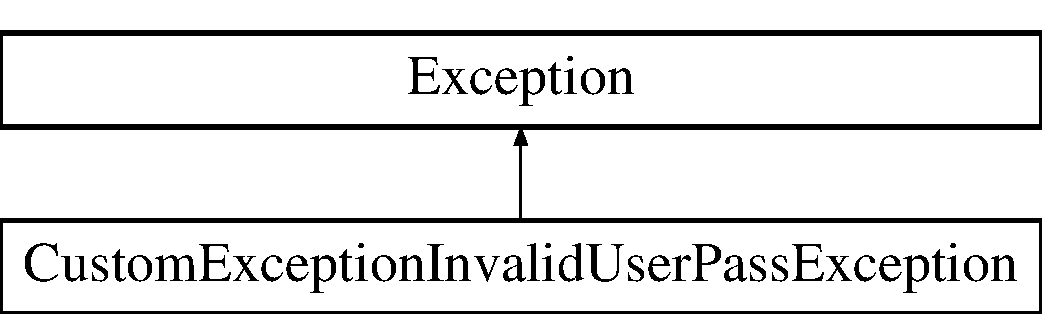
\includegraphics[height=2.000000cm]{class_custom_exception_1_1_invalid_user_pass_exception}
\end{center}
\end{figure}


\subsection{Ausführliche Beschreibung}
Diese Exception wird geworfen wenn der Benutzer nicht vorhanden oder das Passwort falsch ist. 

Definiert in Zeile \hyperlink{_invalid_user_pass_exception_8php_source_l00010}{10} der Datei \hyperlink{_invalid_user_pass_exception_8php_source}{Invalid\-User\-Pass\-Exception.\-php}.



Die Dokumentation für diese Klasse wurde erzeugt aufgrund der Datei\-:\begin{DoxyCompactItemize}
\item 
Invalid\-User\-Pass\-Exception.\-php\end{DoxyCompactItemize}

\hypertarget{class_redirect}{\section{Redirect Klassenreferenz}
\label{class_redirect}\index{Redirect@{Redirect}}
}
\subsection*{Öffentliche, statische Methoden}
\begin{DoxyCompactItemize}
\item 
static \hyperlink{class_redirect_aa19514457e9dddc565309a40f2ecc66c}{Header} (\$url)
\item 
static \hyperlink{class_redirect_a5a8f456a5318387c966b24c0cbe2c083}{to\-Controller} (\$controller)
\end{DoxyCompactItemize}


\subsection{Ausführliche Beschreibung}
\hyperlink{class_redirect}{Redirect} Klasse 

Definiert in Zeile \hyperlink{_redirect_8php_source_l00007}{7} der Datei \hyperlink{_redirect_8php_source}{Redirect.\-php}.



\subsection{Dokumentation der Elementfunktionen}
\hypertarget{class_redirect_aa19514457e9dddc565309a40f2ecc66c}{\index{Redirect@{Redirect}!Header@{Header}}
\index{Header@{Header}!Redirect@{Redirect}}
\subsubsection[{Header}]{\setlength{\rightskip}{0pt plus 5cm}static Redirect\-::\-Header (
\begin{DoxyParamCaption}
\item[{}]{\$url}
\end{DoxyParamCaption}
)\hspace{0.3cm}{\ttfamily [static]}}}\label{class_redirect_aa19514457e9dddc565309a40f2ecc66c}
Header \hyperlink{class_redirect}{Redirect} durchführen


\begin{DoxyParams}[1]{Parameter}
String & {\em \$url} & U\-R\-L \\
\hline
\end{DoxyParams}


Definiert in Zeile \hyperlink{_redirect_8php_source_l00016}{16} der Datei \hyperlink{_redirect_8php_source}{Redirect.\-php}.


\begin{DoxyCode}
00016                                             \{
00017                 
00018                 header(\textcolor{stringliteral}{"Location: $url"});
00019         \}
\end{DoxyCode}
\hypertarget{class_redirect_a5a8f456a5318387c966b24c0cbe2c083}{\index{Redirect@{Redirect}!to\-Controller@{to\-Controller}}
\index{to\-Controller@{to\-Controller}!Redirect@{Redirect}}
\subsubsection[{to\-Controller}]{\setlength{\rightskip}{0pt plus 5cm}static Redirect\-::to\-Controller (
\begin{DoxyParamCaption}
\item[{}]{\$controller}
\end{DoxyParamCaption}
)\hspace{0.3cm}{\ttfamily [static]}}}\label{class_redirect_a5a8f456a5318387c966b24c0cbe2c083}
Controller \hyperlink{class_redirect}{Redirect} durchführen


\begin{DoxyParams}[1]{Parameter}
String & {\em \$controller} & Controllername \\
\hline
\end{DoxyParams}


Definiert in Zeile \hyperlink{_redirect_8php_source_l00028}{28} der Datei \hyperlink{_redirect_8php_source}{Redirect.\-php}.


\begin{DoxyCode}
00028                                                          \{
00029                 
00030                 header(\textcolor{stringliteral}{"Location: index.php?controller=$controller"});
00031         \}
\end{DoxyCode}


Die Dokumentation für diese Klasse wurde erzeugt aufgrund der Datei\-:\begin{DoxyCompactItemize}
\item 
Redirect.\-php\end{DoxyCompactItemize}

\hypertarget{class_session}{\section{Session Klassenreferenz}
\label{class_session}\index{Session@{Session}}
}
\subsection*{Öffentliche Methoden}
\begin{DoxyCompactItemize}
\item 
\hyperlink{class_session_a2da2caf16a5e784a38fb4d8eede4c6fc}{\-\_\-\-\_\-get} (\$key)
\item 
\hyperlink{class_session_a23489b711b32f8820e3a0c78e03cc9b3}{\-\_\-\-\_\-set} (\$key, \$value)
\end{DoxyCompactItemize}
\subsection*{Öffentliche, statische Methoden}
\begin{DoxyCompactItemize}
\item 
\hypertarget{class_session_a8e7c2ae20ee90a0499c48e05cafafccf}{static {\bfseries get\-Instance} ()}\label{class_session_a8e7c2ae20ee90a0499c48e05cafafccf}

\item 
static \hyperlink{class_session_ab5ee063ee1dd4a5026c1b87caf98c9a0}{auth\-User} ()
\item 
static \hyperlink{class_session_a23cee49624385c6af65af96fb1c682f6}{is\-User\-Authed} ()
\item 
static \hyperlink{class_session_a49f0fb7185ab07bdbf6bdff477b43ff8}{is\-User\-Authed\-Check} ()
\item 
static \hyperlink{class_session_a5dde74b6fa44649e5b73cb1096930dd4}{destroy} ()
\end{DoxyCompactItemize}
\subsection*{Private Methoden}
\begin{DoxyCompactItemize}
\item 
\hypertarget{class_session_a09e5dba2aa1cb9edf024641fd7fcec9c}{{\bfseries \-\_\-\-\_\-clone} ()}\label{class_session_a09e5dba2aa1cb9edf024641fd7fcec9c}

\end{DoxyCompactItemize}
\subsection*{Private Attribute}
\begin{DoxyCompactItemize}
\item 
\hypertarget{class_session_ab7f2fef2f9f2501956a7139fdf060397}{{\bfseries \$session} = array()}\label{class_session_ab7f2fef2f9f2501956a7139fdf060397}

\end{DoxyCompactItemize}
\subsection*{Statische, private Attribute}
\begin{DoxyCompactItemize}
\item 
\hypertarget{class_session_a86a6e52b2a48eeafaaff766db1973cef}{static {\bfseries \$instance} = null}\label{class_session_a86a6e52b2a48eeafaaff766db1973cef}

\end{DoxyCompactItemize}


\subsection{Ausführliche Beschreibung}
\hyperlink{class_session}{Session} Klasse als Singleton Pattern

\$session = \-::get\-Instance(); \$session-\/$>$key = \char`\"{}value\char`\"{};

\-::destroy(); 

Definiert in Zeile \hyperlink{_session_8php_source_l00017}{17} der Datei \hyperlink{_session_8php_source}{Session.\-php}.



\subsection{Dokumentation der Elementfunktionen}
\hypertarget{class_session_a2da2caf16a5e784a38fb4d8eede4c6fc}{\index{Session@{Session}!\-\_\-\-\_\-get@{\-\_\-\-\_\-get}}
\index{\-\_\-\-\_\-get@{\-\_\-\-\_\-get}!Session@{Session}}
\subsubsection[{\-\_\-\-\_\-get}]{\setlength{\rightskip}{0pt plus 5cm}Session\-::\-\_\-\-\_\-get (
\begin{DoxyParamCaption}
\item[{}]{\$key}
\end{DoxyParamCaption}
)}}\label{class_session_a2da2caf16a5e784a38fb4d8eede4c6fc}
Getter Methode


\begin{DoxyParams}[1]{Parameter}
String & {\em \$key} & Schlüssel\\
\hline
\end{DoxyParams}
\begin{DoxyReturn}{Rückgabe}
String Wert 
\end{DoxyReturn}


Definiert in Zeile \hyperlink{_session_8php_source_l00046}{46} der Datei \hyperlink{_session_8php_source}{Session.\-php}.


\begin{DoxyCode}
00046                                     \{
00047                                 
00048                 \textcolor{keywordflow}{if} (array\_key\_exists($key, $\_SESSION)) \{
00049                         \textcolor{keywordflow}{return} $\_SESSION;
00050                 \} \textcolor{keywordflow}{else} \{
00051                         \textcolor{keywordflow}{throw} \textcolor{keyword}{new} Exception(\textcolor{stringliteral}{"Session Schluessel '$key' nicht verfuegbar"});
00052                 \}
00053                 
00054         \}
\end{DoxyCode}
\hypertarget{class_session_a23489b711b32f8820e3a0c78e03cc9b3}{\index{Session@{Session}!\-\_\-\-\_\-set@{\-\_\-\-\_\-set}}
\index{\-\_\-\-\_\-set@{\-\_\-\-\_\-set}!Session@{Session}}
\subsubsection[{\-\_\-\-\_\-set}]{\setlength{\rightskip}{0pt plus 5cm}Session\-::\-\_\-\-\_\-set (
\begin{DoxyParamCaption}
\item[{}]{\$key, }
\item[{}]{\$value}
\end{DoxyParamCaption}
)}}\label{class_session_a23489b711b32f8820e3a0c78e03cc9b3}
Setter Methode


\begin{DoxyParams}[1]{Parameter}
String & {\em \$key} & Schlüssel \\
\hline
String & {\em \$value} & Wert \\
\hline
\end{DoxyParams}


Definiert in Zeile \hyperlink{_session_8php_source_l00064}{64} der Datei \hyperlink{_session_8php_source}{Session.\-php}.


\begin{DoxyCode}
00064                                             \{
00065                                 
00066                 $\_SESSION[$key] = $value;
00067                 
00068         \}
\end{DoxyCode}
\hypertarget{class_session_ab5ee063ee1dd4a5026c1b87caf98c9a0}{\index{Session@{Session}!auth\-User@{auth\-User}}
\index{auth\-User@{auth\-User}!Session@{Session}}
\subsubsection[{auth\-User}]{\setlength{\rightskip}{0pt plus 5cm}static Session\-::auth\-User (
\begin{DoxyParamCaption}
{}
\end{DoxyParamCaption}
)\hspace{0.3cm}{\ttfamily [static]}}}\label{class_session_ab5ee063ee1dd4a5026c1b87caf98c9a0}
Benutzer Authentifizeren 

Definiert in Zeile \hyperlink{_session_8php_source_l00075}{75} der Datei \hyperlink{_session_8php_source}{Session.\-php}.


\begin{DoxyCode}
00075                                           \{
00076                 
00077                 $\_SESSION[\textcolor{stringliteral}{'\_\_AUTH'}] = 1;
00078                 
00079         \}
\end{DoxyCode}
\hypertarget{class_session_a5dde74b6fa44649e5b73cb1096930dd4}{\index{Session@{Session}!destroy@{destroy}}
\index{destroy@{destroy}!Session@{Session}}
\subsubsection[{destroy}]{\setlength{\rightskip}{0pt plus 5cm}static Session\-::destroy (
\begin{DoxyParamCaption}
{}
\end{DoxyParamCaption}
)\hspace{0.3cm}{\ttfamily [static]}}}\label{class_session_a5dde74b6fa44649e5b73cb1096930dd4}
\hyperlink{class_session}{Session} loeschen 

Definiert in Zeile \hyperlink{_session_8php_source_l00114}{114} der Datei \hyperlink{_session_8php_source}{Session.\-php}.


\begin{DoxyCode}
00114                                          \{
00115                 
00116                 session\_destroy();
00117                 
00118         \}
\end{DoxyCode}
\hypertarget{class_session_a23cee49624385c6af65af96fb1c682f6}{\index{Session@{Session}!is\-User\-Authed@{is\-User\-Authed}}
\index{is\-User\-Authed@{is\-User\-Authed}!Session@{Session}}
\subsubsection[{is\-User\-Authed}]{\setlength{\rightskip}{0pt plus 5cm}static Session\-::is\-User\-Authed (
\begin{DoxyParamCaption}
{}
\end{DoxyParamCaption}
)\hspace{0.3cm}{\ttfamily [static]}}}\label{class_session_a23cee49624385c6af65af96fb1c682f6}
Ueberprüfen ob Benutzer Authentifiziert ist

\begin{DoxyReturn}{Rückgabe}
Boolean 
\end{DoxyReturn}


Definiert in Zeile \hyperlink{_session_8php_source_l00088}{88} der Datei \hyperlink{_session_8php_source}{Session.\-php}.


\begin{DoxyCode}
00088                                               \{
00089                 
00090                 \textcolor{keywordflow}{if} (array\_key\_exists(\textcolor{stringliteral}{'\_\_AUTH'}, $\_SESSION) && $\_SESSION[\textcolor{stringliteral}{'\_\_AUTH'}] == 1) \textcolor{keywordflow}{return} \textcolor{keyword}{true};
00091                 
00092                 \textcolor{keywordflow}{return} \textcolor{keyword}{false};
00093                 
00094         \}
\end{DoxyCode}
\hypertarget{class_session_a49f0fb7185ab07bdbf6bdff477b43ff8}{\index{Session@{Session}!is\-User\-Authed\-Check@{is\-User\-Authed\-Check}}
\index{is\-User\-Authed\-Check@{is\-User\-Authed\-Check}!Session@{Session}}
\subsubsection[{is\-User\-Authed\-Check}]{\setlength{\rightskip}{0pt plus 5cm}static Session\-::is\-User\-Authed\-Check (
\begin{DoxyParamCaption}
{}
\end{DoxyParamCaption}
)\hspace{0.3cm}{\ttfamily [static]}}}\label{class_session_a49f0fb7185ab07bdbf6bdff477b43ff8}
Ueberprüfen ob Benutzer Authentifiziert ist

Ansonsten Exception werfen 

Definiert in Zeile \hyperlink{_session_8php_source_l00103}{103} der Datei \hyperlink{_session_8php_source}{Session.\-php}.


\begin{DoxyCode}
00103                                                    \{
00104                 
00105                 \textcolor{keywordflow}{if} (!self::isUserAuthed()) \textcolor{keywordflow}{throw} \textcolor{keyword}{new} \hyperlink{class_custom_exception_1_1_user_not_authed_exception}{Ex\(\backslash\)UserNotAuthedException}(\textcolor{stringliteral}{"
      Sie haben keine Berechtigung für diese Seite"});
00106                 
00107         \} 
\end{DoxyCode}


Die Dokumentation für diese Klasse wurde erzeugt aufgrund der Datei\-:\begin{DoxyCompactItemize}
\item 
Session.\-php\end{DoxyCompactItemize}

\hypertarget{class_controller_1_1_admin_1_1_stats}{\section{Controller\textbackslash{}Admin\textbackslash{}Stats Klassenreferenz}
\label{class_controller_1_1_admin_1_1_stats}\index{Controller\textbackslash{}\-Admin\textbackslash{}\-Stats@{Controller\textbackslash{}\-Admin\textbackslash{}\-Stats}}
}
Klassendiagramm für Controller\textbackslash{}Admin\textbackslash{}Stats\-:\begin{figure}[H]
\begin{center}
\leavevmode
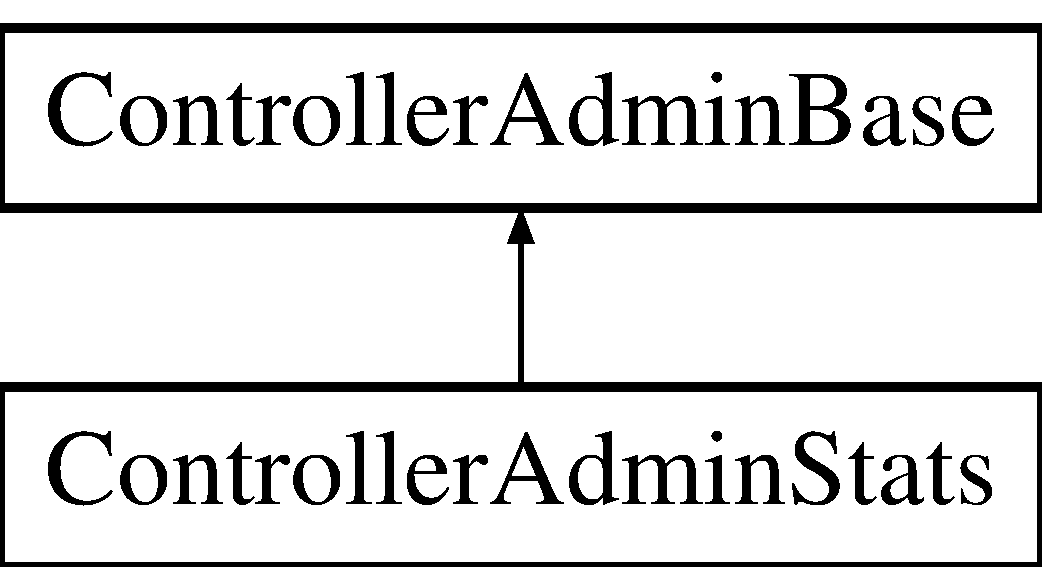
\includegraphics[height=2.000000cm]{class_controller_1_1_admin_1_1_stats}
\end{center}
\end{figure}
\subsection*{Öffentliche Methoden}
\begin{DoxyCompactItemize}
\item 
\hyperlink{class_controller_1_1_admin_1_1_stats_a04ab2733a1fb549ca76f4c78d946f5c7}{Index\-\_\-\-Action} ()
\end{DoxyCompactItemize}


\subsection{Ausführliche Beschreibung}
Admin Statistik Controller 

Definiert in Zeile \hyperlink{_stats_8php_source_l00010}{10} der Datei \hyperlink{_stats_8php_source}{Stats.\-php}.



\subsection{Dokumentation der Elementfunktionen}
\hypertarget{class_controller_1_1_admin_1_1_stats_a04ab2733a1fb549ca76f4c78d946f5c7}{\index{Controller\-::\-Admin\-::\-Stats@{Controller\-::\-Admin\-::\-Stats}!Index\-\_\-\-Action@{Index\-\_\-\-Action}}
\index{Index\-\_\-\-Action@{Index\-\_\-\-Action}!Controller::Admin::Stats@{Controller\-::\-Admin\-::\-Stats}}
\subsubsection[{Index\-\_\-\-Action}]{\setlength{\rightskip}{0pt plus 5cm}Controller\textbackslash{}\-Admin\textbackslash{}\-Stats\-::\-Index\-\_\-\-Action (
\begin{DoxyParamCaption}
{}
\end{DoxyParamCaption}
)}}\label{class_controller_1_1_admin_1_1_stats_a04ab2733a1fb549ca76f4c78d946f5c7}
Default \hyperlink{class_controller_1_1_index}{Index} Get Action 

Definiert in Zeile \hyperlink{_stats_8php_source_l00018}{18} der Datei \hyperlink{_stats_8php_source}{Stats.\-php}.


\begin{DoxyCode}
00018                                        \{
00019                 
00020                 $model = new \(\backslash\)Model\(\backslash\)Survey();
00021                 
00022                 $view = new \(\backslash\)View();
00023                 $view->setTemplate(\textcolor{stringliteral}{'admin\_stats'});
00024                 $view->assign(\textcolor{stringliteral}{'stats'}, $model->getStats());
00025                 $view->display();
00026                 
00027         \}       
\end{DoxyCode}


Die Dokumentation für diese Klasse wurde erzeugt aufgrund der Datei\-:\begin{DoxyCompactItemize}
\item 
Stats.\-php\end{DoxyCompactItemize}

\hypertarget{class_model_1_1_survey}{\section{Model\textbackslash{}Survey Klassenreferenz}
\label{class_model_1_1_survey}\index{Model\textbackslash{}\-Survey@{Model\textbackslash{}\-Survey}}
}
Klassendiagramm für Model\textbackslash{}Survey\-:\begin{figure}[H]
\begin{center}
\leavevmode
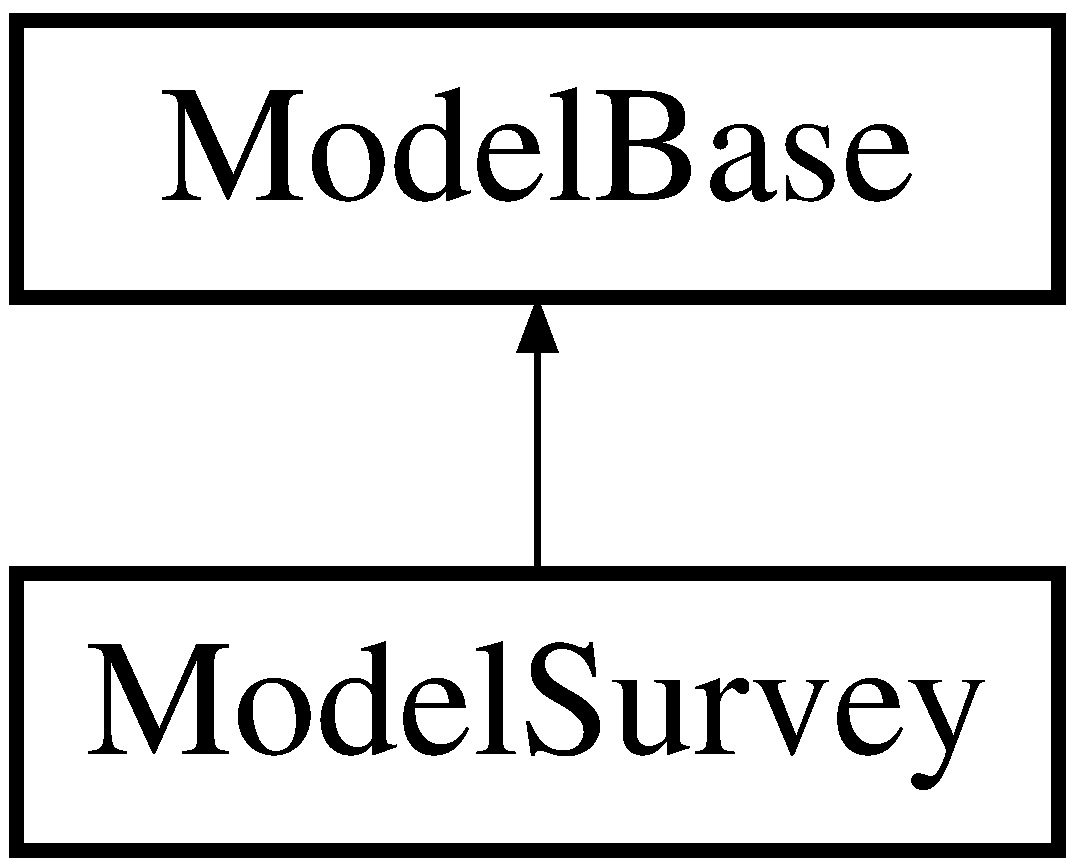
\includegraphics[height=2.000000cm]{class_model_1_1_survey}
\end{center}
\end{figure}
\subsection*{Öffentliche Methoden}
\begin{DoxyCompactItemize}
\item 
\hyperlink{class_model_1_1_survey_a259373a6fdcae5796fc6e14586c98474}{get\-Surveys} ()
\item 
\hyperlink{class_model_1_1_survey_a85d138e55d090b11ba406db39f7d2e72}{get\-Survey\-Name} (\$survey)
\item 
\hyperlink{class_model_1_1_survey_a7f2d5fba208ba0f2ec426db9b9075115}{get\-Survey\-Items} (\$survey)
\item 
\hyperlink{class_model_1_1_survey_ac4b8b489fe806c31bd05d8ec626aae16}{get\-Survey\-Item\-Count} (\$survey)
\item 
\hyperlink{class_model_1_1_survey_a3423f530767905dd0b52858c70d82877}{get\-Survey\-Result} (\$survey)
\item 
\hyperlink{class_model_1_1_survey_ae8dbded81f45b3d84c061bb1bf5ba97f}{get\-Stats} ()
\item 
\hyperlink{class_model_1_1_survey_a39a47b914740e87bc133a72c4721b018}{save\-New\-Answers} (\$answer\-Arr)
\item 
\hyperlink{class_model_1_1_survey_a80276047e075565b781c60d7ac25b3a6}{delete\-Survey} (\$id)
\item 
\hyperlink{class_model_1_1_survey_acf9f6e213e5fd9a31a998db3ddf9026c}{add\-Survey} (\$name, \$answer\-Arr)
\end{DoxyCompactItemize}
\subsection*{Private Methoden}
\begin{DoxyCompactItemize}
\item 
\hyperlink{class_model_1_1_survey_a5c2c5d322a7ae1786acb783f472cc074}{get\-Table\-Count} (\$table)
\end{DoxyCompactItemize}
\subsection*{Weitere Geerbte Elemente}


\subsection{Ausführliche Beschreibung}
Umfrage Datenmodell 

Definiert in Zeile \hyperlink{_model_2_survey_8php_source_l00009}{9} der Datei \hyperlink{_model_2_survey_8php_source}{Model/\-Survey.\-php}.



\subsection{Dokumentation der Elementfunktionen}
\hypertarget{class_model_1_1_survey_acf9f6e213e5fd9a31a998db3ddf9026c}{\index{Model\-::\-Survey@{Model\-::\-Survey}!add\-Survey@{add\-Survey}}
\index{add\-Survey@{add\-Survey}!Model::Survey@{Model\-::\-Survey}}
\subsubsection[{add\-Survey}]{\setlength{\rightskip}{0pt plus 5cm}Model\textbackslash{}\-Survey\-::add\-Survey (
\begin{DoxyParamCaption}
\item[{}]{\$name, }
\item[{}]{\$answer\-Arr}
\end{DoxyParamCaption}
)}}\label{class_model_1_1_survey_acf9f6e213e5fd9a31a998db3ddf9026c}
neue Umfrage hinzufügen


\begin{DoxyParams}[1]{Parameter}
String & {\em \$name} & Name der Umfrage \\
\hline
Array & {\em \$anser\-Arr} & Array mit den möglichen Antworten \\
\hline
\end{DoxyParams}


Definiert in Zeile \hyperlink{_model_2_survey_8php_source_l00167}{167} der Datei \hyperlink{_model_2_survey_8php_source}{Model/\-Survey.\-php}.


\begin{DoxyCode}
00167                                                      \{
00168                 
00169                 \textcolor{keywordflow}{if} (empty($name)) \textcolor{keywordflow}{return};
00170                 
00171                 $stmt = $this->dbh->prepare(\textcolor{stringliteral}{"INSERT INTO Survey SET Name = :name"});
00172                 $stmt->bindParam(\textcolor{stringliteral}{':name'}, $name);
00173                 
00174                 $stmt->execute();
00175 
00176                 $surveyID = $this->dbh->lastInsertId();
00177                 
00178                 $stmt = $this->dbh->prepare(\textcolor{stringliteral}{"INSERT INTO SurveyItems SET Name = :name, SurveyID = :id"});
00179                 
00180                 $stmt->bindParam(\textcolor{stringliteral}{':id'}, $surveyID);
00181 
00182                 \textcolor{keywordflow}{foreach} ($answerArr as $answer) \{
00183 
00184                         \textcolor{keywordflow}{if} (!empty($answer)) \{
00185                                 $stmt->bindParam(\textcolor{stringliteral}{':name'}, $answer);
00186                                 $stmt->execute();
00187                         \}
00188                         
00189                 \}
00190                 
00191         \}
\end{DoxyCode}
\hypertarget{class_model_1_1_survey_a80276047e075565b781c60d7ac25b3a6}{\index{Model\-::\-Survey@{Model\-::\-Survey}!delete\-Survey@{delete\-Survey}}
\index{delete\-Survey@{delete\-Survey}!Model::Survey@{Model\-::\-Survey}}
\subsubsection[{delete\-Survey}]{\setlength{\rightskip}{0pt plus 5cm}Model\textbackslash{}\-Survey\-::delete\-Survey (
\begin{DoxyParamCaption}
\item[{}]{\$id}
\end{DoxyParamCaption}
)}}\label{class_model_1_1_survey_a80276047e075565b781c60d7ac25b3a6}
Umfrage löschen


\begin{DoxyParams}[1]{Parameter}
Integer & {\em \$id} & Umfragen\-I\-D \\
\hline
\end{DoxyParams}


Definiert in Zeile \hyperlink{_model_2_survey_8php_source_l00149}{149} der Datei \hyperlink{_model_2_survey_8php_source}{Model/\-Survey.\-php}.


\begin{DoxyCode}
00149                                           \{
00150                 
00151                 $stmt = $this->dbh->prepare(\textcolor{stringliteral}{"DELETE FROM Survey WHERE ID = :id"});
00152                 $stmt->bindParam(\textcolor{stringliteral}{':id'}, $id);
00153         
00154                 $stmt->execute();
00155                 
00156         \}       
\end{DoxyCode}
\hypertarget{class_model_1_1_survey_ae8dbded81f45b3d84c061bb1bf5ba97f}{\index{Model\-::\-Survey@{Model\-::\-Survey}!get\-Stats@{get\-Stats}}
\index{get\-Stats@{get\-Stats}!Model::Survey@{Model\-::\-Survey}}
\subsubsection[{get\-Stats}]{\setlength{\rightskip}{0pt plus 5cm}Model\textbackslash{}\-Survey\-::get\-Stats (
\begin{DoxyParamCaption}
{}
\end{DoxyParamCaption}
)}}\label{class_model_1_1_survey_ae8dbded81f45b3d84c061bb1bf5ba97f}
Statistiken holen 

Definiert in Zeile \hyperlink{_model_2_survey_8php_source_l00109}{109} der Datei \hyperlink{_model_2_survey_8php_source}{Model/\-Survey.\-php}.


\begin{DoxyCode}
00109                                    \{
00110                 
00111                 $stat = array();
00112 
00113                 $stat[\textcolor{stringliteral}{'user\_cnt'}] = $this->\hyperlink{class_model_1_1_survey_a5c2c5d322a7ae1786acb783f472cc074}{getTableCount}(\textcolor{stringliteral}{"User"});
00114                 $stat[\textcolor{stringliteral}{'survey\_cnt'}] = $this->\hyperlink{class_model_1_1_survey_a5c2c5d322a7ae1786acb783f472cc074}{getTableCount}(\textcolor{stringliteral}{"Survey"});
00115                 $stat[\textcolor{stringliteral}{'survey\_items\_cnt'}] = $this->\hyperlink{class_model_1_1_survey_a5c2c5d322a7ae1786acb783f472cc074}{getTableCount}(\textcolor{stringliteral}{"SurveyItems"});
00116                 $stat[\textcolor{stringliteral}{'answer\_cnt'}] = $this->\hyperlink{class_model_1_1_survey_a5c2c5d322a7ae1786acb783f472cc074}{getTableCount}(\textcolor{stringliteral}{"SurveyAnswer"});
00117                 
00118                 \textcolor{keywordflow}{return} $stat;
00119         \}
\end{DoxyCode}
\hypertarget{class_model_1_1_survey_ac4b8b489fe806c31bd05d8ec626aae16}{\index{Model\-::\-Survey@{Model\-::\-Survey}!get\-Survey\-Item\-Count@{get\-Survey\-Item\-Count}}
\index{get\-Survey\-Item\-Count@{get\-Survey\-Item\-Count}!Model::Survey@{Model\-::\-Survey}}
\subsubsection[{get\-Survey\-Item\-Count}]{\setlength{\rightskip}{0pt plus 5cm}Model\textbackslash{}\-Survey\-::get\-Survey\-Item\-Count (
\begin{DoxyParamCaption}
\item[{}]{\$survey}
\end{DoxyParamCaption}
)}}\label{class_model_1_1_survey_ac4b8b489fe806c31bd05d8ec626aae16}
Anzahl der Abgegeben Umfragewerte


\begin{DoxyParams}[1]{Parameter}
Integer & {\em \$survey} & Umfrage\-Id\\
\hline
\end{DoxyParams}
\begin{DoxyReturn}{Rückgabe}
Integer Anzahl der Ergebnisse zur Umfrage 
\end{DoxyReturn}


Definiert in Zeile \hyperlink{_model_2_survey_8php_source_l00075}{75} der Datei \hyperlink{_model_2_survey_8php_source}{Model/\-Survey.\-php}.


\begin{DoxyCode}
00075                                                     \{
00076                 
00077                 $stmt = $this->dbh->prepare(\textcolor{stringliteral}{"SELECT COUNT(*) AS cnt FROM SurveyAnswer WHERE SurveyItemID IN
       (SELECT ID FROM SurveyItems WHERE SurveyID = :id)"});
00078                 $stmt->bindParam(\textcolor{stringliteral}{':id'}, $survey);
00079                 $stmt->execute();
00080                 $res = $stmt->fetchObject();
00081 
00082                 \textcolor{keywordflow}{return} $res->cnt;
00083         
00084         \}
\end{DoxyCode}
\hypertarget{class_model_1_1_survey_a7f2d5fba208ba0f2ec426db9b9075115}{\index{Model\-::\-Survey@{Model\-::\-Survey}!get\-Survey\-Items@{get\-Survey\-Items}}
\index{get\-Survey\-Items@{get\-Survey\-Items}!Model::Survey@{Model\-::\-Survey}}
\subsubsection[{get\-Survey\-Items}]{\setlength{\rightskip}{0pt plus 5cm}Model\textbackslash{}\-Survey\-::get\-Survey\-Items (
\begin{DoxyParamCaption}
\item[{}]{\$survey}
\end{DoxyParamCaption}
)}}\label{class_model_1_1_survey_a7f2d5fba208ba0f2ec426db9b9075115}
Umfrage Punkte holen


\begin{DoxyParams}[1]{Parameter}
Integer & {\em \$survey} & Umfrage\-Id\\
\hline
\end{DoxyParams}
\begin{DoxyReturn}{Rückgabe}
Array 
\end{DoxyReturn}


Definiert in Zeile \hyperlink{_model_2_survey_8php_source_l00054}{54} der Datei \hyperlink{_model_2_survey_8php_source}{Model/\-Survey.\-php}.


\begin{DoxyCode}
00054                                                 \{
00055                 
00056                 $stmt = $this->dbh->prepare(\textcolor{stringliteral}{"SELECT ID, Name FROM SurveyItems WHERE SurveyID = :id ORDER BY
       Name"});
00057                 $stmt->bindParam(\textcolor{stringliteral}{':id'}, $survey);
00058                 $stmt->execute();
00059                 
00060                 \textcolor{keywordflow}{return} $stmt->fetchAll();
00061 
00062                 
00063                 
00064         \}
\end{DoxyCode}
\hypertarget{class_model_1_1_survey_a85d138e55d090b11ba406db39f7d2e72}{\index{Model\-::\-Survey@{Model\-::\-Survey}!get\-Survey\-Name@{get\-Survey\-Name}}
\index{get\-Survey\-Name@{get\-Survey\-Name}!Model::Survey@{Model\-::\-Survey}}
\subsubsection[{get\-Survey\-Name}]{\setlength{\rightskip}{0pt plus 5cm}Model\textbackslash{}\-Survey\-::get\-Survey\-Name (
\begin{DoxyParamCaption}
\item[{}]{\$survey}
\end{DoxyParamCaption}
)}}\label{class_model_1_1_survey_a85d138e55d090b11ba406db39f7d2e72}
Umfragename holen


\begin{DoxyParams}[1]{Parameter}
Integer & {\em \$survey} & Umfrage\-Id\\
\hline
\end{DoxyParams}
\begin{DoxyReturn}{Rückgabe}
String Name der Umfrage 
\end{DoxyReturn}


Definiert in Zeile \hyperlink{_model_2_survey_8php_source_l00034}{34} der Datei \hyperlink{_model_2_survey_8php_source}{Model/\-Survey.\-php}.


\begin{DoxyCode}
00034                                                \{
00035                 
00036                 $stmt = $this->dbh->prepare(\textcolor{stringliteral}{"SELECT Name FROM Survey WHERE ID = :id"});
00037                 $stmt->bindParam(\textcolor{stringliteral}{':id'}, $survey);
00038                 $stmt->execute();
00039                 $res = $stmt->fetchObject();
00040 
00041                 \textcolor{keywordflow}{return} $res->Name;
00042                 
00043         \}
\end{DoxyCode}
\hypertarget{class_model_1_1_survey_a3423f530767905dd0b52858c70d82877}{\index{Model\-::\-Survey@{Model\-::\-Survey}!get\-Survey\-Result@{get\-Survey\-Result}}
\index{get\-Survey\-Result@{get\-Survey\-Result}!Model::Survey@{Model\-::\-Survey}}
\subsubsection[{get\-Survey\-Result}]{\setlength{\rightskip}{0pt plus 5cm}Model\textbackslash{}\-Survey\-::get\-Survey\-Result (
\begin{DoxyParamCaption}
\item[{}]{\$survey}
\end{DoxyParamCaption}
)}}\label{class_model_1_1_survey_a3423f530767905dd0b52858c70d82877}
Umfrage Ergebnisse holen


\begin{DoxyParams}[1]{Parameter}
Integer & {\em \$survey} & Umfrage\-Id\\
\hline
\end{DoxyParams}
\begin{DoxyReturn}{Rückgabe}
Array 
\end{DoxyReturn}


Definiert in Zeile \hyperlink{_model_2_survey_8php_source_l00094}{94} der Datei \hyperlink{_model_2_survey_8php_source}{Model/\-Survey.\-php}.


\begin{DoxyCode}
00094                                                  \{
00095                 
00096                 $stmt = $this->dbh->prepare(\textcolor{stringliteral}{"SELECT i.Name, COUNT(a.ID) as cnt FROM SurveyItems i LEFT JOIN
       SurveyAnswer a ON i.ID = a. SurveyItemID WHERE i.SurveyID = :id GROUP BY Name ORDER BY i.Name"});
00097                 $stmt->bindParam(\textcolor{stringliteral}{':id'}, $survey);
00098                 $stmt->execute();
00099                 
00100                 \textcolor{keywordflow}{return} $stmt->fetchAll();
00101                 
00102         \}
\end{DoxyCode}
\hypertarget{class_model_1_1_survey_a259373a6fdcae5796fc6e14586c98474}{\index{Model\-::\-Survey@{Model\-::\-Survey}!get\-Surveys@{get\-Surveys}}
\index{get\-Surveys@{get\-Surveys}!Model::Survey@{Model\-::\-Survey}}
\subsubsection[{get\-Surveys}]{\setlength{\rightskip}{0pt plus 5cm}Model\textbackslash{}\-Survey\-::get\-Surveys (
\begin{DoxyParamCaption}
{}
\end{DoxyParamCaption}
)}}\label{class_model_1_1_survey_a259373a6fdcae5796fc6e14586c98474}
Umfragen holen

\begin{DoxyReturn}{Rückgabe}
Array 
\end{DoxyReturn}


Definiert in Zeile \hyperlink{_model_2_survey_8php_source_l00018}{18} der Datei \hyperlink{_model_2_survey_8php_source}{Model/\-Survey.\-php}.


\begin{DoxyCode}
00018                                      \{
00019                 
00020                 $stmt = $this->dbh->query(\textcolor{stringliteral}{"SELECT * FROM Survey"});
00021                 \textcolor{keywordflow}{return} $stmt->fetchAll();       
00022                                 
00023         \}
\end{DoxyCode}
\hypertarget{class_model_1_1_survey_a5c2c5d322a7ae1786acb783f472cc074}{\index{Model\-::\-Survey@{Model\-::\-Survey}!get\-Table\-Count@{get\-Table\-Count}}
\index{get\-Table\-Count@{get\-Table\-Count}!Model::Survey@{Model\-::\-Survey}}
\subsubsection[{get\-Table\-Count}]{\setlength{\rightskip}{0pt plus 5cm}Model\textbackslash{}\-Survey\-::get\-Table\-Count (
\begin{DoxyParamCaption}
\item[{}]{\$table}
\end{DoxyParamCaption}
)\hspace{0.3cm}{\ttfamily [private]}}}\label{class_model_1_1_survey_a5c2c5d322a7ae1786acb783f472cc074}
Anzahl der Tupel zurückgeben


\begin{DoxyParams}[1]{Parameter}
String & {\em \$table} & Tabellenname\\
\hline
\end{DoxyParams}
\begin{DoxyReturn}{Rückgabe}
Integer Anzahl der Tupel 
\end{DoxyReturn}


Definiert in Zeile \hyperlink{_model_2_survey_8php_source_l00202}{202} der Datei \hyperlink{_model_2_survey_8php_source}{Model/\-Survey.\-php}.


\begin{DoxyCode}
00202                                                \{
00203                 
00204                 
00205                 \textcolor{keywordflow}{switch} ($table) \{
00206                         
00207                         \textcolor{keywordflow}{case} \textcolor{stringliteral}{"User"}:
00208                         \textcolor{keywordflow}{case} \textcolor{stringliteral}{"Survey"}:
00209                         \textcolor{keywordflow}{case} \textcolor{stringliteral}{"SurveyItems"}:     
00210                         \textcolor{keywordflow}{case} \textcolor{stringliteral}{"SurveyAnswer"}:
00211                                 $stmt = $this->dbh->query(\textcolor{stringliteral}{"SELECT COUNT(*) AS cnt FROM $table"});
00212                                 \textcolor{keywordflow}{return} $stmt->fetchObject()->cnt;       
00213                                 \textcolor{keywordflow}{break};  
00214                         \textcolor{keywordflow}{default}:
00215                                 \textcolor{keywordflow}{throw} new \(\backslash\)Exception(\textcolor{stringliteral}{"Illegaler Tabellenname $table"});
00216                                 
00217                 \}
00218                                 
00219         \}
\end{DoxyCode}
\hypertarget{class_model_1_1_survey_a39a47b914740e87bc133a72c4721b018}{\index{Model\-::\-Survey@{Model\-::\-Survey}!save\-New\-Answers@{save\-New\-Answers}}
\index{save\-New\-Answers@{save\-New\-Answers}!Model::Survey@{Model\-::\-Survey}}
\subsubsection[{save\-New\-Answers}]{\setlength{\rightskip}{0pt plus 5cm}Model\textbackslash{}\-Survey\-::save\-New\-Answers (
\begin{DoxyParamCaption}
\item[{}]{\$answer\-Arr}
\end{DoxyParamCaption}
)}}\label{class_model_1_1_survey_a39a47b914740e87bc133a72c4721b018}
Antworten Speichern


\begin{DoxyParams}[1]{Parameter}
Integer & {\em \$answer\-Arr} & Array mit den Antwort I\-Ds \\
\hline
\end{DoxyParams}


Definiert in Zeile \hyperlink{_model_2_survey_8php_source_l00128}{128} der Datei \hyperlink{_model_2_survey_8php_source}{Model/\-Survey.\-php}.


\begin{DoxyCode}
00128                                                    \{
00129 
00130                 $stmt = $this->dbh->prepare(\textcolor{stringliteral}{"INSERT INTO SurveyAnswer SET SurveyItemID = :id"});
00131                 
00132                 \textcolor{keywordflow}{foreach} ($answerArr as $answer) \{
00133 
00134                                 $stmt->bindParam(\textcolor{stringliteral}{':id'}, $answer);
00135                                 $stmt->execute();       
00136                         
00137                 \}
00138         
00139         \}
\end{DoxyCode}


Die Dokumentation für diese Klasse wurde erzeugt aufgrund der Datei\-:\begin{DoxyCompactItemize}
\item 
Model/\-Survey.\-php\end{DoxyCompactItemize}

\hypertarget{class_controller_1_1_admin_1_1_survey}{\section{Controller\textbackslash{}Admin\textbackslash{}Survey Klassenreferenz}
\label{class_controller_1_1_admin_1_1_survey}\index{Controller\textbackslash{}\-Admin\textbackslash{}\-Survey@{Controller\textbackslash{}\-Admin\textbackslash{}\-Survey}}
}
Klassendiagramm für Controller\textbackslash{}Admin\textbackslash{}Survey\-:\begin{figure}[H]
\begin{center}
\leavevmode
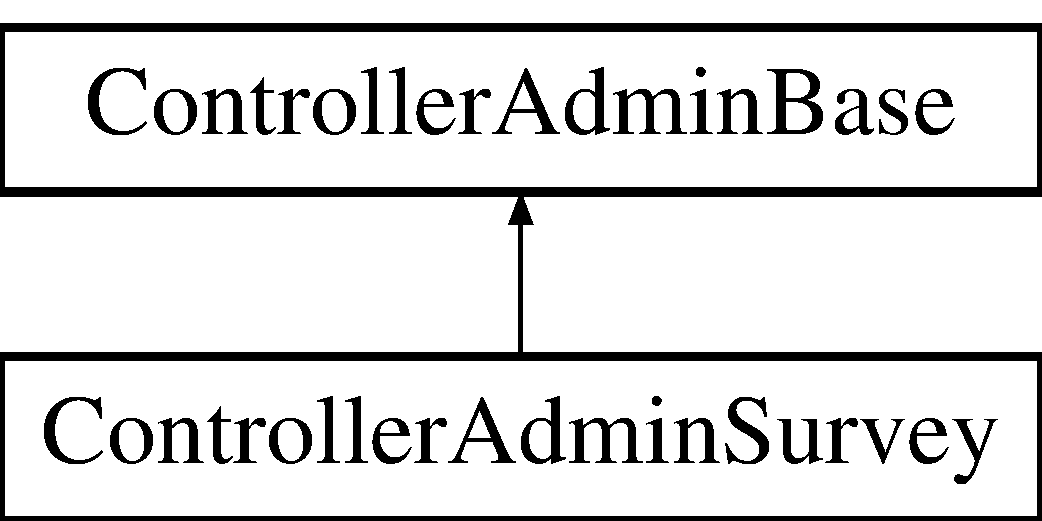
\includegraphics[height=2.000000cm]{class_controller_1_1_admin_1_1_survey}
\end{center}
\end{figure}
\subsection*{Öffentliche Methoden}
\begin{DoxyCompactItemize}
\item 
\hyperlink{class_controller_1_1_admin_1_1_survey_ab79ba5fab3d2048a72c71fcd3176dd72}{Index\-\_\-\-Action} ()
\item 
\hyperlink{class_controller_1_1_admin_1_1_survey_a618d9d0d906df279c7b34ae9458fa977}{Add\-\_\-\-P\-O\-S\-T\-\_\-\-Action} ()
\end{DoxyCompactItemize}


\subsection{Ausführliche Beschreibung}
Admin Umfrage Controller 

Definiert in Zeile \hyperlink{_controller_2_admin_2_survey_8php_source_l00010}{10} der Datei \hyperlink{_controller_2_admin_2_survey_8php_source}{Controller/\-Admin/\-Survey.\-php}.



\subsection{Dokumentation der Elementfunktionen}
\hypertarget{class_controller_1_1_admin_1_1_survey_a618d9d0d906df279c7b34ae9458fa977}{\index{Controller\-::\-Admin\-::\-Survey@{Controller\-::\-Admin\-::\-Survey}!Add\-\_\-\-P\-O\-S\-T\-\_\-\-Action@{Add\-\_\-\-P\-O\-S\-T\-\_\-\-Action}}
\index{Add\-\_\-\-P\-O\-S\-T\-\_\-\-Action@{Add\-\_\-\-P\-O\-S\-T\-\_\-\-Action}!Controller::Admin::Survey@{Controller\-::\-Admin\-::\-Survey}}
\subsubsection[{Add\-\_\-\-P\-O\-S\-T\-\_\-\-Action}]{\setlength{\rightskip}{0pt plus 5cm}Controller\textbackslash{}\-Admin\textbackslash{}\-Survey\-::\-Add\-\_\-\-P\-O\-S\-T\-\_\-\-Action (
\begin{DoxyParamCaption}
{}
\end{DoxyParamCaption}
)}}\label{class_controller_1_1_admin_1_1_survey_a618d9d0d906df279c7b34ae9458fa977}
neue Umfragen hinzufügen 

Definiert in Zeile \hyperlink{_controller_2_admin_2_survey_8php_source_l00033}{33} der Datei \hyperlink{_controller_2_admin_2_survey_8php_source}{Controller/\-Admin/\-Survey.\-php}.


\begin{DoxyCode}
00033                                           \{
00034                 
00035                 $this->\hyperlink{class_controller_1_1_admin_1_1_survey_ab79ba5fab3d2048a72c71fcd3176dd72}{Index\_Action}();
00036                 
00037         \}
\end{DoxyCode}
\hypertarget{class_controller_1_1_admin_1_1_survey_ab79ba5fab3d2048a72c71fcd3176dd72}{\index{Controller\-::\-Admin\-::\-Survey@{Controller\-::\-Admin\-::\-Survey}!Index\-\_\-\-Action@{Index\-\_\-\-Action}}
\index{Index\-\_\-\-Action@{Index\-\_\-\-Action}!Controller::Admin::Survey@{Controller\-::\-Admin\-::\-Survey}}
\subsubsection[{Index\-\_\-\-Action}]{\setlength{\rightskip}{0pt plus 5cm}Controller\textbackslash{}\-Admin\textbackslash{}\-Survey\-::\-Index\-\_\-\-Action (
\begin{DoxyParamCaption}
{}
\end{DoxyParamCaption}
)}}\label{class_controller_1_1_admin_1_1_survey_ab79ba5fab3d2048a72c71fcd3176dd72}
Default \hyperlink{class_controller_1_1_index}{Index} Get Action 

Definiert in Zeile \hyperlink{_controller_2_admin_2_survey_8php_source_l00017}{17} der Datei \hyperlink{_controller_2_admin_2_survey_8php_source}{Controller/\-Admin/\-Survey.\-php}.


\begin{DoxyCode}
00017                                        \{
00018                 
00019                 $model = new \(\backslash\)Model\(\backslash\)Survey();
00020                 
00021                 $view = new \(\backslash\)View();
00022                 $view->setTemplate(\textcolor{stringliteral}{'admin\_surveys'});
00023                 $view->assign(\textcolor{stringliteral}{'surveys'}, $model->getSurveys());
00024                 $view->display();
00025                 
00026         \}       
\end{DoxyCode}


Die Dokumentation für diese Klasse wurde erzeugt aufgrund der Datei\-:\begin{DoxyCompactItemize}
\item 
Controller/\-Admin/\-Survey.\-php\end{DoxyCompactItemize}

\hypertarget{class_controller_1_1_survey}{\section{Controller\textbackslash{}Survey Klassenreferenz}
\label{class_controller_1_1_survey}\index{Controller\textbackslash{}\-Survey@{Controller\textbackslash{}\-Survey}}
}
\subsection*{Öffentliche Methoden}
\begin{DoxyCompactItemize}
\item 
\hyperlink{class_controller_1_1_survey_a96fc5091aa3b11390854987ecf667f15}{\-\_\-\-\_\-construct} ()
\item 
\hyperlink{class_controller_1_1_survey_ab9a687bf4e1fe3c36b13ff873e94b212}{Index\-\_\-\-Action} ()
\item 
\hyperlink{class_controller_1_1_survey_a1a671d9a36a993bab69c12c16fcc60cc}{Save\-\_\-\-P\-O\-S\-T\-\_\-\-Action} ()
\end{DoxyCompactItemize}
\subsection*{Private Attribute}
\begin{DoxyCompactItemize}
\item 
\hypertarget{class_controller_1_1_survey_af4dfeefe4184d06ce16596852d1699fe}{{\bfseries \$view}}\label{class_controller_1_1_survey_af4dfeefe4184d06ce16596852d1699fe}

\item 
\hypertarget{class_controller_1_1_survey_aaf7d79f033911a2dccb8a9b86335f608}{{\bfseries \$model}}\label{class_controller_1_1_survey_aaf7d79f033911a2dccb8a9b86335f608}

\item 
\hypertarget{class_controller_1_1_survey_a5dbe38a79e94073188649d98023be07f}{{\bfseries \$survey}}\label{class_controller_1_1_survey_a5dbe38a79e94073188649d98023be07f}

\end{DoxyCompactItemize}


\subsection{Ausführliche Beschreibung}
Umfrage Controller 

Definiert in Zeile \hyperlink{_controller_2_survey_8php_source_l00010}{10} der Datei \hyperlink{_controller_2_survey_8php_source}{Controller/\-Survey.\-php}.



\subsection{Beschreibung der Konstruktoren und Destruktoren}
\hypertarget{class_controller_1_1_survey_a96fc5091aa3b11390854987ecf667f15}{\index{Controller\-::\-Survey@{Controller\-::\-Survey}!\-\_\-\-\_\-construct@{\-\_\-\-\_\-construct}}
\index{\-\_\-\-\_\-construct@{\-\_\-\-\_\-construct}!Controller::Survey@{Controller\-::\-Survey}}
\subsubsection[{\-\_\-\-\_\-construct}]{\setlength{\rightskip}{0pt plus 5cm}Controller\textbackslash{}\-Survey\-::\-\_\-\-\_\-construct (
\begin{DoxyParamCaption}
{}
\end{DoxyParamCaption}
)}}\label{class_controller_1_1_survey_a96fc5091aa3b11390854987ecf667f15}
Kontruktor 

Definiert in Zeile \hyperlink{_controller_2_survey_8php_source_l00021}{21} der Datei \hyperlink{_controller_2_survey_8php_source}{Controller/\-Survey.\-php}.


\begin{DoxyCode}
00021                                       \{
00022                 
00023                 $this->view = new \(\backslash\)View();
00024                 $this->model = new \(\backslash\)Model\(\backslash\)Survey();
00025                 $this->survey = intval($\_GET[\textcolor{stringliteral}{'survey'}]);
00026                 
00027         \}
\end{DoxyCode}


\subsection{Dokumentation der Elementfunktionen}
\hypertarget{class_controller_1_1_survey_ab9a687bf4e1fe3c36b13ff873e94b212}{\index{Controller\-::\-Survey@{Controller\-::\-Survey}!Index\-\_\-\-Action@{Index\-\_\-\-Action}}
\index{Index\-\_\-\-Action@{Index\-\_\-\-Action}!Controller::Survey@{Controller\-::\-Survey}}
\subsubsection[{Index\-\_\-\-Action}]{\setlength{\rightskip}{0pt plus 5cm}Controller\textbackslash{}\-Survey\-::\-Index\-\_\-\-Action (
\begin{DoxyParamCaption}
{}
\end{DoxyParamCaption}
)}}\label{class_controller_1_1_survey_ab9a687bf4e1fe3c36b13ff873e94b212}
Default \hyperlink{class_controller_1_1_index}{Index} Get Action 

Definiert in Zeile \hyperlink{_controller_2_survey_8php_source_l00034}{34} der Datei \hyperlink{_controller_2_survey_8php_source}{Controller/\-Survey.\-php}.


\begin{DoxyCode}
00034                                        \{
00035                 
00036 
00037 
00038                 \textcolor{keywordflow}{if} ($this->survey == 0) \{
00039                         
00040                         $this->view->setTemplate(\textcolor{stringliteral}{'surveys'});
00041                         $this->view->assign(\textcolor{stringliteral}{'surveys'}, $this->model->getSurveys());
00042                         $this->view->display();
00043                                                 
00044                 \} \textcolor{keywordflow}{else} \{
00045 
00046                         $this->view->setTemplate(\textcolor{stringliteral}{'survey'});
00047                         $this->view->assign(\textcolor{stringliteral}{'survey\_id'}, $this->survey);
00048                         $this->view->assign(\textcolor{stringliteral}{'survey\_name'}, $this->model->getSurveyName($this->survey));
00049                         $this->view->assign(\textcolor{stringliteral}{'survey\_items'}, $this->model->getSurveyItems($this->survey));
00050                         $this->view->display();
00051         
00052                         
00053                 \}
00054                 
00055         \}
\end{DoxyCode}
\hypertarget{class_controller_1_1_survey_a1a671d9a36a993bab69c12c16fcc60cc}{\index{Controller\-::\-Survey@{Controller\-::\-Survey}!Save\-\_\-\-P\-O\-S\-T\-\_\-\-Action@{Save\-\_\-\-P\-O\-S\-T\-\_\-\-Action}}
\index{Save\-\_\-\-P\-O\-S\-T\-\_\-\-Action@{Save\-\_\-\-P\-O\-S\-T\-\_\-\-Action}!Controller::Survey@{Controller\-::\-Survey}}
\subsubsection[{Save\-\_\-\-P\-O\-S\-T\-\_\-\-Action}]{\setlength{\rightskip}{0pt plus 5cm}Controller\textbackslash{}\-Survey\-::\-Save\-\_\-\-P\-O\-S\-T\-\_\-\-Action (
\begin{DoxyParamCaption}
{}
\end{DoxyParamCaption}
)}}\label{class_controller_1_1_survey_a1a671d9a36a993bab69c12c16fcc60cc}
Umfrage Ergebnisse speichern

Auswertung anzeigen 

Definiert in Zeile \hyperlink{_controller_2_survey_8php_source_l00064}{64} der Datei \hyperlink{_controller_2_survey_8php_source}{Controller/\-Survey.\-php}.


\begin{DoxyCode}
00064                                            \{
00065 
00066                 $this->view->setTemplate(\textcolor{stringliteral}{'survey\_result'});
00067                 $this->view->assign(\textcolor{stringliteral}{'survey\_name'}, $this->model->getSurveyName($this->survey));
00068                 $this->view->assign(\textcolor{stringliteral}{'survey\_cnt'}, $this->model->getSurveyItemCount($this->survey));
00069                 $this->view->assign(\textcolor{stringliteral}{'survey\_result'}, $this->model->getSurveyResult($this->survey));
00070                 $this->view->display();
00071                                 
00072         \}
\end{DoxyCode}


Die Dokumentation für diese Klasse wurde erzeugt aufgrund der Datei\-:\begin{DoxyCompactItemize}
\item 
Controller/\-Survey.\-php\end{DoxyCompactItemize}

\hypertarget{class_controller_1_1_admin_1_1_user}{\section{Controller\textbackslash{}Admin\textbackslash{}User Klassenreferenz}
\label{class_controller_1_1_admin_1_1_user}\index{Controller\textbackslash{}\-Admin\textbackslash{}\-User@{Controller\textbackslash{}\-Admin\textbackslash{}\-User}}
}
Klassendiagramm für Controller\textbackslash{}Admin\textbackslash{}User\-:\begin{figure}[H]
\begin{center}
\leavevmode
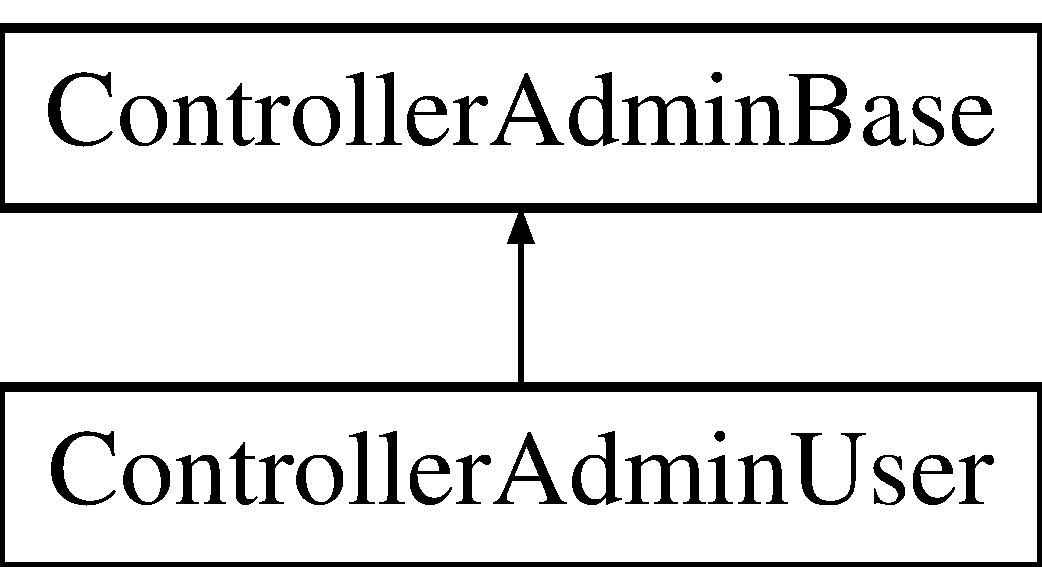
\includegraphics[height=2.000000cm]{class_controller_1_1_admin_1_1_user}
\end{center}
\end{figure}
\subsection*{Öffentliche Methoden}
\begin{DoxyCompactItemize}
\item 
\hyperlink{class_controller_1_1_admin_1_1_user_acbbf0aeb45206f2d0c9e347e8a1d19c9}{\-\_\-\-\_\-construct} ()
\item 
\hyperlink{class_controller_1_1_admin_1_1_user_a006c1efe9d23f5307039c1beb0ce18a5}{Index\-\_\-\-Action} ()
\item 
\hyperlink{class_controller_1_1_admin_1_1_user_a381c8672d1cec6440138d0bf939fb5ec}{Add\-\_\-\-P\-O\-S\-T\-\_\-\-Action} ()
\item 
\hyperlink{class_controller_1_1_admin_1_1_user_a96952a534cf944ff774fdab36d8efaaa}{Delete\-\_\-\-Action} ()
\end{DoxyCompactItemize}
\subsection*{Weitere Geerbte Elemente}


\subsection{Ausführliche Beschreibung}
Admin Benutzer Controller 

Definiert in Zeile \hyperlink{_controller_2_admin_2_user_8php_source_l00010}{10} der Datei \hyperlink{_controller_2_admin_2_user_8php_source}{Controller/\-Admin/\-User.\-php}.



\subsection{Beschreibung der Konstruktoren und Destruktoren}
\hypertarget{class_controller_1_1_admin_1_1_user_acbbf0aeb45206f2d0c9e347e8a1d19c9}{\index{Controller\-::\-Admin\-::\-User@{Controller\-::\-Admin\-::\-User}!\-\_\-\-\_\-construct@{\-\_\-\-\_\-construct}}
\index{\-\_\-\-\_\-construct@{\-\_\-\-\_\-construct}!Controller::Admin::User@{Controller\-::\-Admin\-::\-User}}
\subsubsection[{\-\_\-\-\_\-construct}]{\setlength{\rightskip}{0pt plus 5cm}Controller\textbackslash{}\-Admin\textbackslash{}\-User\-::\-\_\-\-\_\-construct (
\begin{DoxyParamCaption}
{}
\end{DoxyParamCaption}
)}}\label{class_controller_1_1_admin_1_1_user_acbbf0aeb45206f2d0c9e347e8a1d19c9}
Modell initialisieren 

Definiert in Zeile \hyperlink{_controller_2_admin_2_user_8php_source_l00018}{18} der Datei \hyperlink{_controller_2_admin_2_user_8php_source}{Controller/\-Admin/\-User.\-php}.


\begin{DoxyCode}
00018                                       \{
00019                 
00020                 $this->model = new \(\backslash\)Model\(\backslash\)User();
00021                 
00022                 parent::\_\_construct();
00023         
00024         \}
\end{DoxyCode}


\subsection{Dokumentation der Elementfunktionen}
\hypertarget{class_controller_1_1_admin_1_1_user_a381c8672d1cec6440138d0bf939fb5ec}{\index{Controller\-::\-Admin\-::\-User@{Controller\-::\-Admin\-::\-User}!Add\-\_\-\-P\-O\-S\-T\-\_\-\-Action@{Add\-\_\-\-P\-O\-S\-T\-\_\-\-Action}}
\index{Add\-\_\-\-P\-O\-S\-T\-\_\-\-Action@{Add\-\_\-\-P\-O\-S\-T\-\_\-\-Action}!Controller::Admin::User@{Controller\-::\-Admin\-::\-User}}
\subsubsection[{Add\-\_\-\-P\-O\-S\-T\-\_\-\-Action}]{\setlength{\rightskip}{0pt plus 5cm}Controller\textbackslash{}\-Admin\textbackslash{}\-User\-::\-Add\-\_\-\-P\-O\-S\-T\-\_\-\-Action (
\begin{DoxyParamCaption}
{}
\end{DoxyParamCaption}
)}}\label{class_controller_1_1_admin_1_1_user_a381c8672d1cec6440138d0bf939fb5ec}
Benutzer hinzufuegen 

Definiert in Zeile \hyperlink{_controller_2_admin_2_user_8php_source_l00045}{45} der Datei \hyperlink{_controller_2_admin_2_user_8php_source}{Controller/\-Admin/\-User.\-php}.


\begin{DoxyCode}
00045                                           \{
00046                 
00047                 \textcolor{keywordflow}{if} (isset($\_POST[\textcolor{stringliteral}{'name'}]) && isset($\_POST[\textcolor{stringliteral}{'pass'}])) \{
00048 
00049                         $name = $\_POST[\textcolor{stringliteral}{'name'}];
00050                         $pass = $\_POST[\textcolor{stringliteral}{'pass'}];
00051 
00052                         $this->model->addUser($name, $pass);
00053                         
00054                         $this->\hyperlink{class_controller_1_1_admin_1_1_user_a006c1efe9d23f5307039c1beb0ce18a5}{Index\_Action}();
00055                         
00056                 \} \textcolor{keywordflow}{else} \{
00057                         
00058                         \textcolor{keywordflow}{throw} new \(\backslash\)Exception(\textcolor{stringliteral}{"Illegaler Aufruf"});
00059                         
00060                 \}
00061 
00062                 
00063         \}
\end{DoxyCode}
\hypertarget{class_controller_1_1_admin_1_1_user_a96952a534cf944ff774fdab36d8efaaa}{\index{Controller\-::\-Admin\-::\-User@{Controller\-::\-Admin\-::\-User}!Delete\-\_\-\-Action@{Delete\-\_\-\-Action}}
\index{Delete\-\_\-\-Action@{Delete\-\_\-\-Action}!Controller::Admin::User@{Controller\-::\-Admin\-::\-User}}
\subsubsection[{Delete\-\_\-\-Action}]{\setlength{\rightskip}{0pt plus 5cm}Controller\textbackslash{}\-Admin\textbackslash{}\-User\-::\-Delete\-\_\-\-Action (
\begin{DoxyParamCaption}
{}
\end{DoxyParamCaption}
)}}\label{class_controller_1_1_admin_1_1_user_a96952a534cf944ff774fdab36d8efaaa}
Benutzer loeschen 

Definiert in Zeile \hyperlink{_controller_2_admin_2_user_8php_source_l00070}{70} der Datei \hyperlink{_controller_2_admin_2_user_8php_source}{Controller/\-Admin/\-User.\-php}.


\begin{DoxyCode}
00070                                         \{
00071                 
00072                 
00073                 \textcolor{keywordflow}{if} (isset($\_GET[\textcolor{stringliteral}{'user'}])) \{
00074                         
00075                         $id = intval($\_GET[\textcolor{stringliteral}{'user'}]);
00076 
00077                         \textcolor{keywordflow}{if} ($id > 0) \{
00078                                 
00079                                 $this->model->deleteUser($id);
00080                                                 
00081                                 $this->\hyperlink{class_controller_1_1_admin_1_1_user_a006c1efe9d23f5307039c1beb0ce18a5}{Index\_Action}();                              
00082                         
00083                         \} \textcolor{keywordflow}{else} \{
00084                                 
00085                                 \textcolor{keywordflow}{throw} new \(\backslash\)Exception(\textcolor{stringliteral}{"Illegaler Aufruf"});
00086                                 
00087                         \}
00088                                                 
00089         
00090                 \} \textcolor{keywordflow}{else} \{
00091                         
00092                         \textcolor{keywordflow}{throw} new \(\backslash\)Exception(\textcolor{stringliteral}{"Illegaler Aufruf"});
00093                         
00094                 \}
00095         \}
\end{DoxyCode}
\hypertarget{class_controller_1_1_admin_1_1_user_a006c1efe9d23f5307039c1beb0ce18a5}{\index{Controller\-::\-Admin\-::\-User@{Controller\-::\-Admin\-::\-User}!Index\-\_\-\-Action@{Index\-\_\-\-Action}}
\index{Index\-\_\-\-Action@{Index\-\_\-\-Action}!Controller::Admin::User@{Controller\-::\-Admin\-::\-User}}
\subsubsection[{Index\-\_\-\-Action}]{\setlength{\rightskip}{0pt plus 5cm}Controller\textbackslash{}\-Admin\textbackslash{}\-User\-::\-Index\-\_\-\-Action (
\begin{DoxyParamCaption}
{}
\end{DoxyParamCaption}
)}}\label{class_controller_1_1_admin_1_1_user_a006c1efe9d23f5307039c1beb0ce18a5}
Default \hyperlink{class_controller_1_1_index}{Index} Get Action 

Definiert in Zeile \hyperlink{_controller_2_admin_2_user_8php_source_l00031}{31} der Datei \hyperlink{_controller_2_admin_2_user_8php_source}{Controller/\-Admin/\-User.\-php}.


\begin{DoxyCode}
00031                                        \{
00032                 
00033                 $this->view->setTemplate(\textcolor{stringliteral}{'admin\_user'});
00034                 $this->view->assign(\textcolor{stringliteral}{'users'}, $this->model->getUsers());
00035                 
00036                 $this->view->display();
00037                 
00038         \}       
\end{DoxyCode}


Die Dokumentation für diese Klasse wurde erzeugt aufgrund der Datei\-:\begin{DoxyCompactItemize}
\item 
Controller/\-Admin/\-User.\-php\end{DoxyCompactItemize}

\hypertarget{class_model_1_1_user}{\section{Model\textbackslash{}User Klassenreferenz}
\label{class_model_1_1_user}\index{Model\textbackslash{}\-User@{Model\textbackslash{}\-User}}
}
\subsection*{Öffentliche Methoden}
\begin{DoxyCompactItemize}
\item 
\hyperlink{class_model_1_1_user_a6f75fbb91daa84c817340a254bd1aa6f}{check\-Credentials} (\$user, \$pass)
\item 
\hyperlink{class_model_1_1_user_a306c9d8207c01a0dc603dd3fa148094c}{get\-Users} ()
\end{DoxyCompactItemize}


\subsection{Ausführliche Beschreibung}
Benutzer Datenmodell 

Definiert in Zeile \hyperlink{_model_2_user_8php_source_l00009}{9} der Datei \hyperlink{_model_2_user_8php_source}{Model/\-User.\-php}.



\subsection{Dokumentation der Elementfunktionen}
\hypertarget{class_model_1_1_user_a6f75fbb91daa84c817340a254bd1aa6f}{\index{Model\-::\-User@{Model\-::\-User}!check\-Credentials@{check\-Credentials}}
\index{check\-Credentials@{check\-Credentials}!Model::User@{Model\-::\-User}}
\subsubsection[{check\-Credentials}]{\setlength{\rightskip}{0pt plus 5cm}Model\textbackslash{}\-User\-::check\-Credentials (
\begin{DoxyParamCaption}
\item[{}]{\$user, }
\item[{}]{\$pass}
\end{DoxyParamCaption}
)}}\label{class_model_1_1_user_a6f75fbb91daa84c817340a254bd1aa6f}
Berechtigung ueberprüfen


\begin{DoxyParams}[1]{Parameter}
String & {\em \$user} & Benutzername \\
\hline
String & {\em \$pass} & Passwort\\
\hline
\end{DoxyParams}
\begin{DoxyReturn}{Rückgabe}
Boolean 
\end{DoxyReturn}


Definiert in Zeile \hyperlink{_model_2_user_8php_source_l00022}{22} der Datei \hyperlink{_model_2_user_8php_source}{Model/\-User.\-php}.


\begin{DoxyCode}
00022                                                        \{
00023                 
00024                 \textcolor{keywordflow}{return} \textcolor{keyword}{true};
00025                 
00026         \}
\end{DoxyCode}
\hypertarget{class_model_1_1_user_a306c9d8207c01a0dc603dd3fa148094c}{\index{Model\-::\-User@{Model\-::\-User}!get\-Users@{get\-Users}}
\index{get\-Users@{get\-Users}!Model::User@{Model\-::\-User}}
\subsubsection[{get\-Users}]{\setlength{\rightskip}{0pt plus 5cm}Model\textbackslash{}\-User\-::get\-Users (
\begin{DoxyParamCaption}
{}
\end{DoxyParamCaption}
)}}\label{class_model_1_1_user_a306c9d8207c01a0dc603dd3fa148094c}
Benutzer holen

\begin{DoxyReturn}{Rückgabe}
Array 
\end{DoxyReturn}


Definiert in Zeile \hyperlink{_model_2_user_8php_source_l00035}{35} der Datei \hyperlink{_model_2_user_8php_source}{Model/\-User.\-php}.


\begin{DoxyCode}
00035                                    \{
00036                 
00037                 \textcolor{keywordflow}{return} array(\textcolor{stringliteral}{"sepp"} => date(\textcolor{stringliteral}{"d.m.Y H:i"}, time()), \textcolor{stringliteral}{"franz"} => date(\textcolor{stringliteral}{"d.m.Y H:i"}, time()), \textcolor{stringliteral}{"
      test"} => date(\textcolor{stringliteral}{"d.m.Y H:i"}, time()));
00038         \}
\end{DoxyCode}


Die Dokumentation für diese Klasse wurde erzeugt aufgrund der Datei\-:\begin{DoxyCompactItemize}
\item 
Model/\-User.\-php\end{DoxyCompactItemize}

\hypertarget{class_custom_exception_1_1_user_not_authed_exception}{\section{Custom\-Exception\textbackslash{}User\-Not\-Authed\-Exception Klassenreferenz}
\label{class_custom_exception_1_1_user_not_authed_exception}\index{Custom\-Exception\textbackslash{}\-User\-Not\-Authed\-Exception@{Custom\-Exception\textbackslash{}\-User\-Not\-Authed\-Exception}}
}
Klassendiagramm für Custom\-Exception\textbackslash{}User\-Not\-Authed\-Exception\-:\begin{figure}[H]
\begin{center}
\leavevmode
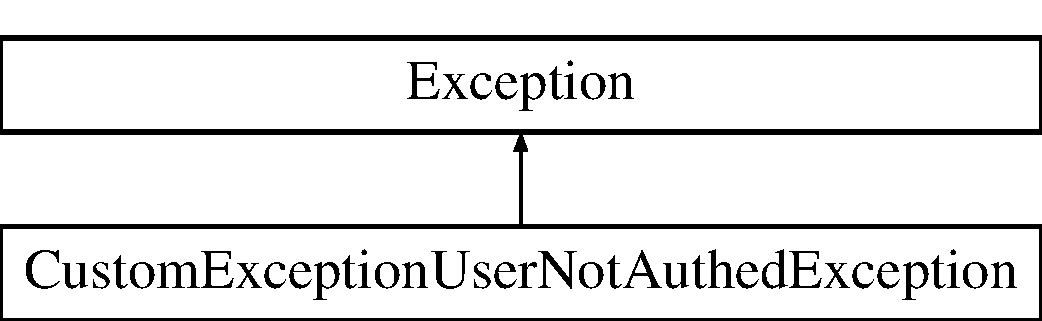
\includegraphics[height=2.000000cm]{class_custom_exception_1_1_user_not_authed_exception}
\end{center}
\end{figure}


\subsection{Ausführliche Beschreibung}
Diese Exception wird geworfen wenn der Benutzer nicht eingeloggt ist. 

Definiert in Zeile \hyperlink{_user_not_authed_exception_8php_source_l00010}{10} der Datei \hyperlink{_user_not_authed_exception_8php_source}{User\-Not\-Authed\-Exception.\-php}.



Die Dokumentation für diese Klasse wurde erzeugt aufgrund der Datei\-:\begin{DoxyCompactItemize}
\item 
User\-Not\-Authed\-Exception.\-php\end{DoxyCompactItemize}

\hypertarget{class_controller_1_1_user_session}{\section{Controller\textbackslash{}User\-Session Klassenreferenz}
\label{class_controller_1_1_user_session}\index{Controller\textbackslash{}\-User\-Session@{Controller\textbackslash{}\-User\-Session}}
}
\subsection*{Öffentliche Methoden}
\begin{DoxyCompactItemize}
\item 
\hyperlink{class_controller_1_1_user_session_a3ab4801a36620e4a99cf3066970ebaf4}{Login\-\_\-\-Action} ()
\item 
\hyperlink{class_controller_1_1_user_session_a0b902f49ccbff4387dcf5655874cbb1c}{Login\-\_\-\-P\-O\-S\-T\-\_\-\-Action} ()
\item 
\hyperlink{class_controller_1_1_user_session_a2078537fe028f203be44fdfe2b3c0036}{Logout\-\_\-\-Action} ()
\end{DoxyCompactItemize}


\subsection{Ausführliche Beschreibung}
Login Controller 

Definiert in Zeile \hyperlink{_user_session_8php_source_l00010}{10} der Datei \hyperlink{_user_session_8php_source}{User\-Session.\-php}.



\subsection{Dokumentation der Elementfunktionen}
\hypertarget{class_controller_1_1_user_session_a3ab4801a36620e4a99cf3066970ebaf4}{\index{Controller\-::\-User\-Session@{Controller\-::\-User\-Session}!Login\-\_\-\-Action@{Login\-\_\-\-Action}}
\index{Login\-\_\-\-Action@{Login\-\_\-\-Action}!Controller::UserSession@{Controller\-::\-User\-Session}}
\subsubsection[{Login\-\_\-\-Action}]{\setlength{\rightskip}{0pt plus 5cm}Controller\textbackslash{}\-User\-Session\-::\-Login\-\_\-\-Action (
\begin{DoxyParamCaption}
{}
\end{DoxyParamCaption}
)}}\label{class_controller_1_1_user_session_a3ab4801a36620e4a99cf3066970ebaf4}
Login Formular anzeigen 

Definiert in Zeile \hyperlink{_user_session_8php_source_l00018}{18} der Datei \hyperlink{_user_session_8php_source}{User\-Session.\-php}.


\begin{DoxyCode}
00018                                        \{
00019 
00020                 $view = new \(\backslash\)View();
00021                 $view->setTemplate(\textcolor{stringliteral}{'login'});
00022                 $view->display();
00023 
00024                 
00025         \}
\end{DoxyCode}
\hypertarget{class_controller_1_1_user_session_a0b902f49ccbff4387dcf5655874cbb1c}{\index{Controller\-::\-User\-Session@{Controller\-::\-User\-Session}!Login\-\_\-\-P\-O\-S\-T\-\_\-\-Action@{Login\-\_\-\-P\-O\-S\-T\-\_\-\-Action}}
\index{Login\-\_\-\-P\-O\-S\-T\-\_\-\-Action@{Login\-\_\-\-P\-O\-S\-T\-\_\-\-Action}!Controller::UserSession@{Controller\-::\-User\-Session}}
\subsubsection[{Login\-\_\-\-P\-O\-S\-T\-\_\-\-Action}]{\setlength{\rightskip}{0pt plus 5cm}Controller\textbackslash{}\-User\-Session\-::\-Login\-\_\-\-P\-O\-S\-T\-\_\-\-Action (
\begin{DoxyParamCaption}
{}
\end{DoxyParamCaption}
)}}\label{class_controller_1_1_user_session_a0b902f49ccbff4387dcf5655874cbb1c}
Verarbeitung der Logindaten 

Definiert in Zeile \hyperlink{_user_session_8php_source_l00032}{32} der Datei \hyperlink{_user_session_8php_source}{User\-Session.\-php}.


\begin{DoxyCode}
00032                                             \{
00033                 
00034                 $user = $\_GET[\textcolor{stringliteral}{'user'}];
00035                 $pass = $\_GET[\textcolor{stringliteral}{'pass'}];
00036                 
00037                 $model = new \(\backslash\)Model\(\backslash\)User();
00038                         
00039                 \textcolor{keywordflow}{if} ($model->checkCredentials($user, $pass)) \{
00040 
00041                         \hyperlink{class_session_ab5ee063ee1dd4a5026c1b87caf98c9a0}{\(\backslash\)Session::authUser}();
00042                         \hyperlink{class_redirect_a5a8f456a5318387c966b24c0cbe2c083}{\(\backslash\)Redirect::toController}(\textcolor{stringliteral}{"Index"});
00043 
00044                 \} \textcolor{keywordflow}{else} \{
00045                 
00046                         $this->\hyperlink{class_controller_1_1_user_session_a3ab4801a36620e4a99cf3066970ebaf4}{Login\_Action}();                      
00047                         
00048                 \}
00049 
00050                 
00051         \}
\end{DoxyCode}
\hypertarget{class_controller_1_1_user_session_a2078537fe028f203be44fdfe2b3c0036}{\index{Controller\-::\-User\-Session@{Controller\-::\-User\-Session}!Logout\-\_\-\-Action@{Logout\-\_\-\-Action}}
\index{Logout\-\_\-\-Action@{Logout\-\_\-\-Action}!Controller::UserSession@{Controller\-::\-User\-Session}}
\subsubsection[{Logout\-\_\-\-Action}]{\setlength{\rightskip}{0pt plus 5cm}Controller\textbackslash{}\-User\-Session\-::\-Logout\-\_\-\-Action (
\begin{DoxyParamCaption}
{}
\end{DoxyParamCaption}
)}}\label{class_controller_1_1_user_session_a2078537fe028f203be44fdfe2b3c0036}
Logout Action 

Definiert in Zeile \hyperlink{_user_session_8php_source_l00058}{58} der Datei \hyperlink{_user_session_8php_source}{User\-Session.\-php}.


\begin{DoxyCode}
00058                                         \{
00059 
00060                 \hyperlink{class_session_a5dde74b6fa44649e5b73cb1096930dd4}{\(\backslash\)Session::destroy}();
00061                 \hyperlink{class_redirect_a5a8f456a5318387c966b24c0cbe2c083}{\(\backslash\)Redirect::toController}(\textcolor{stringliteral}{"Index"});
00062                 
00063         \}
\end{DoxyCode}


Die Dokumentation für diese Klasse wurde erzeugt aufgrund der Datei\-:\begin{DoxyCompactItemize}
\item 
User\-Session.\-php\end{DoxyCompactItemize}

\hypertarget{class_view}{\section{View Klassenreferenz}
\label{class_view}\index{View@{View}}
}
\subsection*{Öffentliche Methoden}
\begin{DoxyCompactItemize}
\item 
\hyperlink{class_view_a2c338778c398ef0e4040bc377242611a}{assign} (\$key, \$value)
\item 
\hyperlink{class_view_a956eb733dd01bd0c42f06d71e11afef3}{set\-Template} (\$template)
\item 
\hyperlink{class_view_a0924100c5e1690a4150bb1c446859e07}{display} ()
\end{DoxyCompactItemize}
\subsection*{Private Methoden}
\begin{DoxyCompactItemize}
\item 
\hyperlink{class_view_a157300b213657f283da80e7430d9e98b}{get\-Template\-On\-Filesystem} (\$template)
\end{DoxyCompactItemize}
\subsection*{Private Attribute}
\begin{DoxyCompactItemize}
\item 
\hypertarget{class_view_a46020b2880e3138be7fd04e0a2a2944f}{{\bfseries \$template\-Path} = 'templates'}\label{class_view_a46020b2880e3138be7fd04e0a2a2944f}

\item 
\hypertarget{class_view_a4833469062d3f9086f204d4be985e9bc}{{\bfseries \$template} = 'index'}\label{class_view_a4833469062d3f9086f204d4be985e9bc}

\item 
\hypertarget{class_view_a6f6d4ba4ff5891b9fcaabf5ab1a888cd}{{\bfseries \$layouttemplate} = '\-\_\-layout'}\label{class_view_a6f6d4ba4ff5891b9fcaabf5ab1a888cd}

\item 
\hypertarget{class_view_add138b1b1fd0769b37c5338f2aa1316d}{{\bfseries \$includetemplate}}\label{class_view_add138b1b1fd0769b37c5338f2aa1316d}

\item 
\hypertarget{class_view_ad4ffe360a4edcdce1cf6abe276f1370f}{{\bfseries \$view} = array()}\label{class_view_ad4ffe360a4edcdce1cf6abe276f1370f}

\end{DoxyCompactItemize}


\subsection{Ausführliche Beschreibung}
\hyperlink{class_view}{View} Klasse 

Definiert in Zeile \hyperlink{_view_8php_source_l00007}{7} der Datei \hyperlink{_view_8php_source}{View.\-php}.



\subsection{Dokumentation der Elementfunktionen}
\hypertarget{class_view_a2c338778c398ef0e4040bc377242611a}{\index{View@{View}!assign@{assign}}
\index{assign@{assign}!View@{View}}
\subsubsection[{assign}]{\setlength{\rightskip}{0pt plus 5cm}View\-::assign (
\begin{DoxyParamCaption}
\item[{}]{\$key, }
\item[{}]{\$value}
\end{DoxyParamCaption}
)}}\label{class_view_a2c338778c398ef0e4040bc377242611a}
Template Variable zuweisen


\begin{DoxyParams}[1]{Parameter}
String & {\em \$key} & Schlüssel \\
\hline
String & {\em \$value} & Wert \\
\hline
\end{DoxyParams}


Definiert in Zeile \hyperlink{_view_8php_source_l00029}{29} der Datei \hyperlink{_view_8php_source}{View.\-php}.


\begin{DoxyCode}
00029                                              \{
00030                 $this->view[$key] = $value;  
00031         \}               
\end{DoxyCode}
\hypertarget{class_view_a0924100c5e1690a4150bb1c446859e07}{\index{View@{View}!display@{display}}
\index{display@{display}!View@{View}}
\subsubsection[{display}]{\setlength{\rightskip}{0pt plus 5cm}View\-::display (
\begin{DoxyParamCaption}
{}
\end{DoxyParamCaption}
)}}\label{class_view_a0924100c5e1690a4150bb1c446859e07}
Template anzeigen 

Definiert in Zeile \hyperlink{_view_8php_source_l00049}{49} der Datei \hyperlink{_view_8php_source}{View.\-php}.


\begin{DoxyCode}
00049                                   \{
00050                 
00051                 $this->includetemplate = $this->\hyperlink{class_view_a157300b213657f283da80e7430d9e98b}{getTemplateOnFilesystem}($this->\textcolor{keyword}{
      template});
00052                 
00053                 \textcolor{comment}{// Überprüfen ob das angeforderte Template Exitiert}
00054                 \textcolor{keywordflow}{if} (file\_exists($this->includetemplate)) \{
00055                         \textcolor{comment}{// Layouttemplate einbinden}
00056                         include $this->\hyperlink{class_view_a157300b213657f283da80e7430d9e98b}{getTemplateOnFilesystem}($this->layouttemplate
      );
00057                         
00058                 \} \textcolor{keywordflow}{else} \{
00059                         
00060                         \textcolor{keywordflow}{throw} \textcolor{keyword}{new} Exception(\textcolor{stringliteral}{"Template '\{$this->template\}' nicht gefunden"});
00061                         
00062                 \}
00063                         
00064         \}
\end{DoxyCode}
\hypertarget{class_view_a157300b213657f283da80e7430d9e98b}{\index{View@{View}!get\-Template\-On\-Filesystem@{get\-Template\-On\-Filesystem}}
\index{get\-Template\-On\-Filesystem@{get\-Template\-On\-Filesystem}!View@{View}}
\subsubsection[{get\-Template\-On\-Filesystem}]{\setlength{\rightskip}{0pt plus 5cm}View\-::get\-Template\-On\-Filesystem (
\begin{DoxyParamCaption}
\item[{}]{\$template}
\end{DoxyParamCaption}
)\hspace{0.3cm}{\ttfamily [private]}}}\label{class_view_a157300b213657f283da80e7430d9e98b}
Anhand des Templatenamen den vollen Pfad inkl Datei zurückgeben


\begin{DoxyParams}[1]{Parameter}
String & {\em \$template} & Templatename\\
\hline
\end{DoxyParams}
\begin{DoxyReturn}{Rückgabe}
String Pfad inkl Dateiname zum Template 
\end{DoxyReturn}


Definiert in Zeile \hyperlink{_view_8php_source_l00075}{75} der Datei \hyperlink{_view_8php_source}{View.\-php}.


\begin{DoxyCode}
00075                                                                  \{
00076                 
00077                 \textcolor{keywordflow}{return} $this->templatePath . DIRECTORY\_SEPARATOR . $template . \textcolor{stringliteral}{".tpl.php"};
00078                 
00079         \}       
\end{DoxyCode}
\hypertarget{class_view_a956eb733dd01bd0c42f06d71e11afef3}{\index{View@{View}!set\-Template@{set\-Template}}
\index{set\-Template@{set\-Template}!View@{View}}
\subsubsection[{set\-Template}]{\setlength{\rightskip}{0pt plus 5cm}View\-::set\-Template (
\begin{DoxyParamCaption}
\item[{}]{\$template}
\end{DoxyParamCaption}
)}}\label{class_view_a956eb733dd01bd0c42f06d71e11afef3}
Template setzen


\begin{DoxyParams}[1]{Parameter}
String & {\em \$template} & Templatename \\
\hline
\end{DoxyParams}


Definiert in Zeile \hyperlink{_view_8php_source_l00040}{40} der Datei \hyperlink{_view_8php_source}{View.\-php}.


\begin{DoxyCode}
00040                                                \{
00041                 $this->\textcolor{keyword}{template} = $template;  
00042         \}  
\end{DoxyCode}


Die Dokumentation für diese Klasse wurde erzeugt aufgrund der Datei\-:\begin{DoxyCompactItemize}
\item 
View.\-php\end{DoxyCompactItemize}

%--- End generated contents ---

% Index
\newpage
\phantomsection
\addcontentsline{toc}{part}{Index}
\printindex

\end{document}
